\chapter{Caracterización de impactos con Deep Learning}

Como se ha mencionado en la introducción, el objetivo de la segunda herramienta es la localización de impactos.\\

C. Aguilar en \cite{Christian_TFM} utilizó algoritmos de triangulación para localizar impactos en placas de material compuesto. Para ello, recogió los diferentes tiempos de llegada de las ondas de Lamb provocadas por el impacto con cada uno de los piezoeléctricos integrados en la estructura. Utilizando el campo de velocidades sobre la estructura y el tiempo de llegada a los diferentes piezoeléctricos, se puede obtener la posición del impacto. 

Los materiales compuestos tienen propiedades anisótropas, por lo que la velocidad de propagación de las ondas por el material no es igual en todas las direcciones. Esto hizo que en \cite{Christian_TFM} se tuviera que calcular el campo de velocidades sobre la placa rigidizada.\\

La herramienta que se quiere desarrollar en este estudio busca localizar impactos en estructuras complejas fabricadas en material compuesto. En la Figura \ref{fig:costilla_ala} se puede ver un ejemplo de este tipo de estructuras. Esta complejidad hace inviable la utilización de algoritmos de triangulación por la dificultad de calcular campo de velocidades, entonces se abre la puerta a la utilización de Deep Learning para este fin.

\begin{figure}[h!]
    \centering
    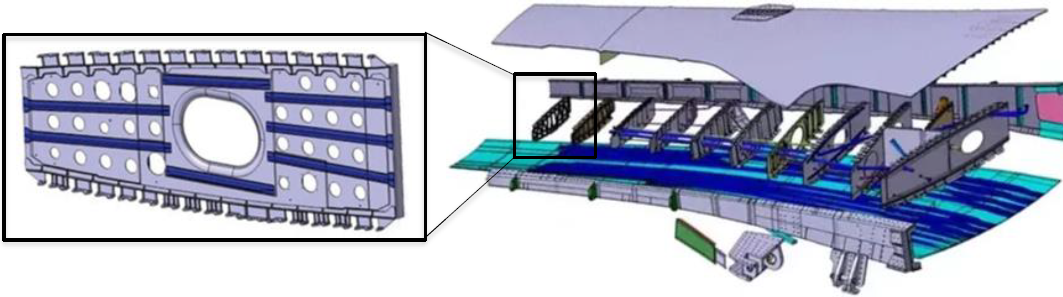
\includegraphics[width=135mm, angle=0]{4/Fotos/costilla_ala.png}
    \captionsetup{justification=centering,margin=1.25cm}
    \caption{Costillas en una semiala del Airbus A380}
    \label{fig:costilla_ala}
\end{figure}

La estructura que se va a utilizar en este estudio es un cuarto de costilla del Airbus A380. En la Figura \ref{fig:costilla_piezos} se puede apreciar la complejidad de la estructura con múltiples vaciados y rigidizadores. También se ven los piezoeléctricos encargados de recoger las ondas de Lamb provocadas por los impactos.\\

\begin{figure}[h!]
    \centering
    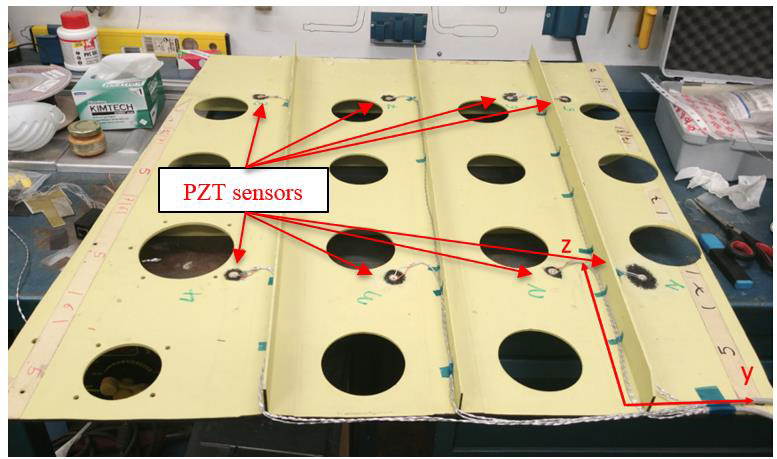
\includegraphics[width=125mm, angle=0]{4/Fotos/costilla_piezos.png}
    \captionsetup{justification=centering,margin=1.25cm}
    \caption{Estructura en estudio instrumentada}
    \label{fig:costilla_piezos}
\end{figure}

Como se ha visto anteriormente, las NN clasificadoreas dan un resultado discreto, en forma de clases. Para que la red pueda clasificar, se ha discretizado la superficie de la costilla en diferentes celdas, cuyos índices serán considerados las clases. Esta discretización se puede ver en la Figura \ref{fig:costilla_celdas} junto con la posición de los piezoeléctricos.

\begin{figure}[h!]
    \centering
    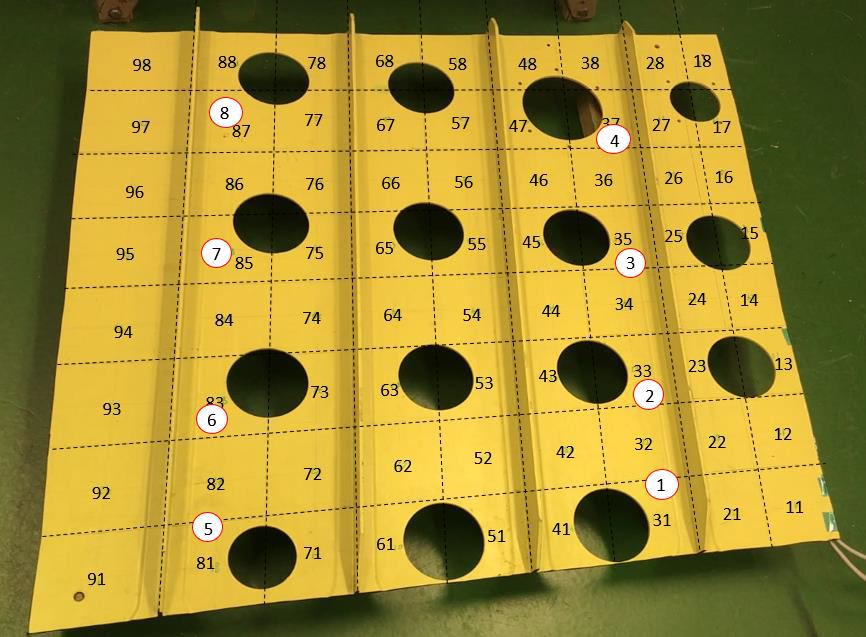
\includegraphics[width=125mm, angle=0]{4/Fotos/costilla_celdas.png}
    \captionsetup{justification=centering,margin=1.25cm}
    \caption{Discretización de la superficie de la costilla}
    \label{fig:costilla_celdas}
\end{figure}

Al igual que para las redes de detección de daño, se necesita un Data Set con una cantidad de muestras del orden de $10^3$ por clase. El realizar una cantidad tan elevada de impactos de forma manual y precisa no es viable, lo que ha llevado a plantear dos métodos diferentes de obtención de impactos que se desarrollarán en este punto:

\begin{itemize}
    \item[$\bullet$] Impactador automático
    \item[$\bullet$] Generación de impactos con redes tipo Generative Adversarial Networks (GANs)
\end{itemize}

Una vez se hayan conseguido los impactos, se creará una nueva red que tendrá como objetivo clasificar un impacto en las celdas de la costilla.

%  -----------------------------------------  %

\section{Impactador automático (SI TE PARECE BIEN)}

Una forma muy eficiente de realizar una tarea repetitiva es mediante su automatización, sobre todo si se requiere un nivel alto de precisión durante todo el proceso. Para entrenar a las redes neuronales es necesario una gran cantidad de impactos para cada celda, cuanta mayor cantidad de impactos e incluso, cuanta mayor dispersión dentro cada celda, mejor clasificará ante nuevos impactos que no han formado parte del proceso de entrenamiento de la red.\\

Para llevar a cabo el diseño se necesitan definir una serie de requisitos que el modelo final deberá cumplir. 

    \subsection{Impactador estructura}

% -- -- %

    \subsection{Electrónica - Software y hardware}

% -- -- %

    \subsection{Adquisición y procesado de datos}

\clearpage


%  -----------------------------------------  %


\section{Generative Adversarial Networks}

Muchos algoritmos de Machine Learning tienen como entrada datos complejos (una imagen, por ejemplo) y generan una salida simple (la clase avión). Sin embargo, el objetivo de un modelo generativo es completamente opuesto. A partir de una entrada simple, como puede ser un vector de números aleatorios, generar como salida una imágen realista de un avión.

Las Generative Adversarial Networks (GANs) son un tipo de modelo generativo muy efectivo, creado en el 2014 por Ian J. Goodfellow \cite{GANs}, que ha suscitado un gran interés en la comunidad de ML.\\

Un concepto importante de las GANs es que utiliza la aleatoriedad como instrumento creador. Esto hace que cuando introduzcas una entrada aleatoria nunca genere una imagen repetida, ya que hay muy pocas probabilidades de generar dos grupos de datos aleatorios iguales.

Pero igual de importante es que pensar en términos de probabilidades también nos ayuda a traducir el problema de la generación de imágenes en un marco matemático natural. Obviamente no se quieren elegir imágenes uniformemente al azar, ya que eso sólo produciría ruido. En su lugar, queremos que el sistema aprenda qué imágenes tienen probabilidades de ser caras, y cuáles no. Matemáticamente, esto implica modelar una distribución de probabilidad en las imágenes, es decir, una función que diga qué imágenes son probables de ser caras y cuáles no. Este tipo de problema se puede entender como modelar una función en un espacio de altas dimensiones y es exactamente el tipo de cosas para las que están hechas las redes neuronales.\\

La gran idea que define a una GAN es establecer este problema de modelización como una especie de concurso. De aquí viene la parte "adversaria" del nombre. La idea clave es construir no una, sino dos redes enfrentadas: un generador y un discriminador. El generador trata de crear salidas sintéticas aleatorias (por ejemplo, imágenes de rostros), mientras que el discriminador trata de diferenciarlas de las salidas reales (por ejemplo, una base de datos de famosos). El objetivo es que a medida que las dos redes se enfrenten, ambas mejoren cada vez más, con el resultado final de una red generadora que produzca salidas realistas.

En resumen: Las redes generadoras adversarias son redes neuronales que aprenden a elegir muestras de una distribución especial (la parte "generativa" del nombre), y lo hacen estableciendo una competencia (por lo tanto "adversaria"). 

Esta idea de dos redes enfrentadas se puede ver en la Figura \ref{fig:gan_arquitectura}

\begin{figure}[h!]
    \centering
    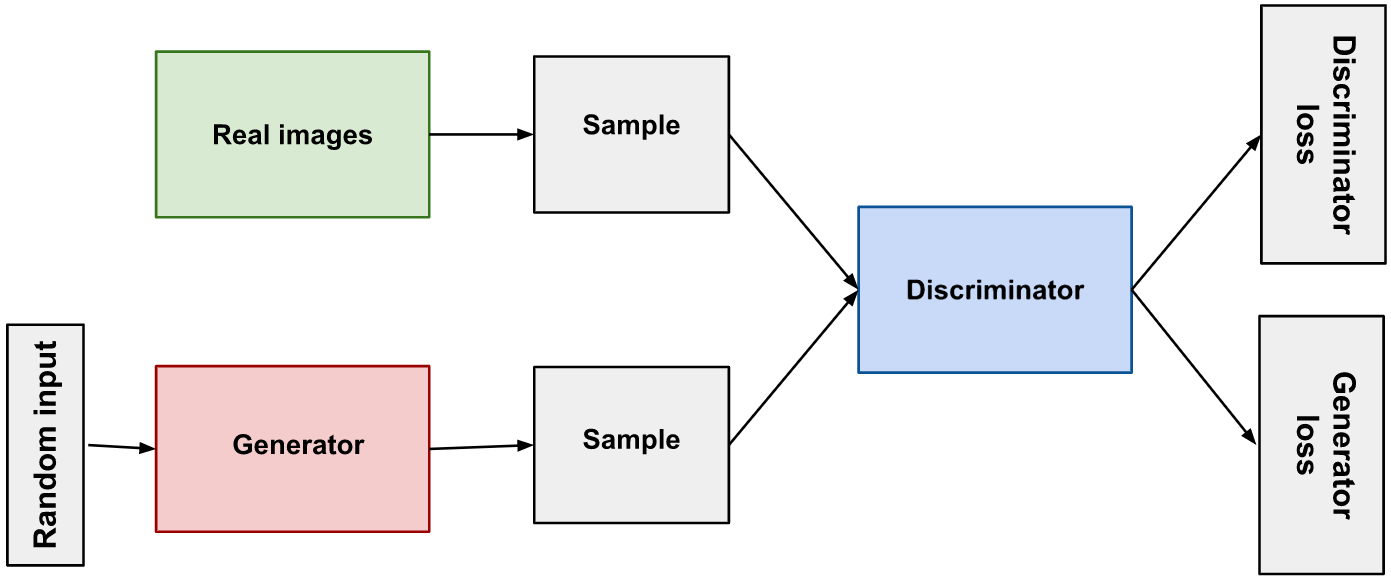
\includegraphics[width=125mm, angle=0]{4/Fotos/gan_representacion.png}
    \captionsetup{justification=centering,margin=1.25cm}
    \caption{Representación simplificada de la aquitectura de una red GAN}
    \label{fig:gan_arquitectura}
\end{figure}

Descripción extraída de \cite{GAN_lab}\\

En este estudio no se tiene como objetivo crear imágenes realistas, sino impactos que sean similares a los que se recogieron en \cite{Christian_TFM}. Para entender mejor la forma de los datos que se van a utilizar se han representado varias muestras en la Figura \ref{fig:multiple_impactos}. Cada muestra consta de las medidas de tensión (voltios) recogidas por los ocho piezoeléctricos en una ventana de tiempo de 0.0125 segundos. Este tipo de datos se puede clasificar como series de datos temporales multivariable.

Si se presta atención a las subfiguras \ref{fig:celda_11_1} y \ref{fig:celda_11_2} puede apreciarse que, aun siendo un impacto en la misma celda, las mediciones son muy dispares. Recuperando la idea de que una parte esencial en las GANs es que se generan los nuevos impactos a partir de datos aleatorios, el que haya variación dentro de impactos en una misma celda facilita a la red el aprendizaje y, por lo tanto, el generar impactos más similares a los reales.

\begin{figure}[h!]
 \centering
  \subfloat[Muestra 1 de impacto en celda 11]{
    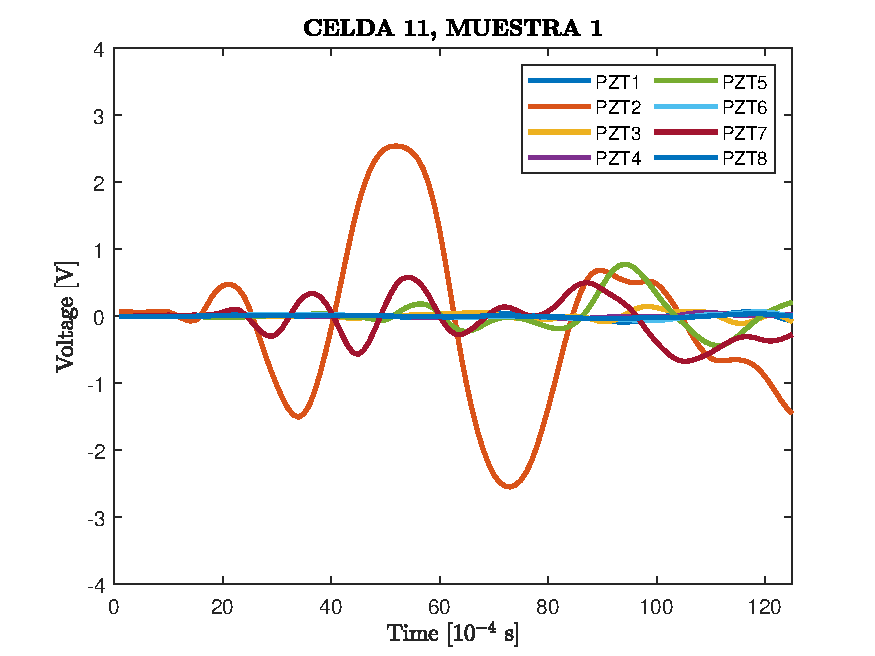
\includegraphics[width=75mm]{4/Fotos/Impacto_11_1.pdf}
    \label{fig:celda_11_1}}
  \subfloat[Muestra 2 de impacto en celda 11]{
    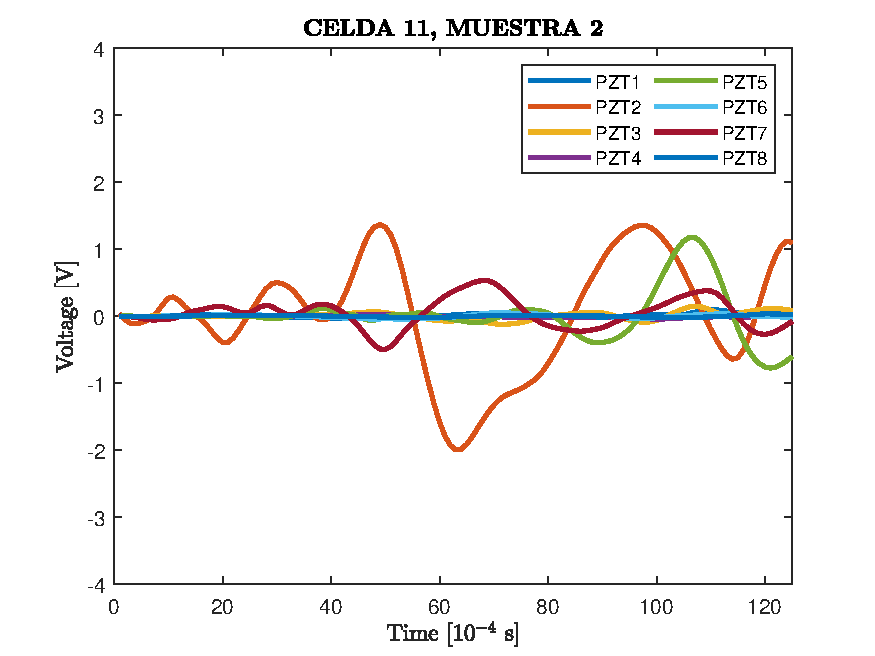
\includegraphics[width=75mm]{4/Fotos/Impacto_11_2.pdf}
    \label{fig:celda_11_2}}
    \label{Esto solo esta aqui para separar en dos bloques}
  \subfloat[Muestra 1 de impacto en celda 72]{
    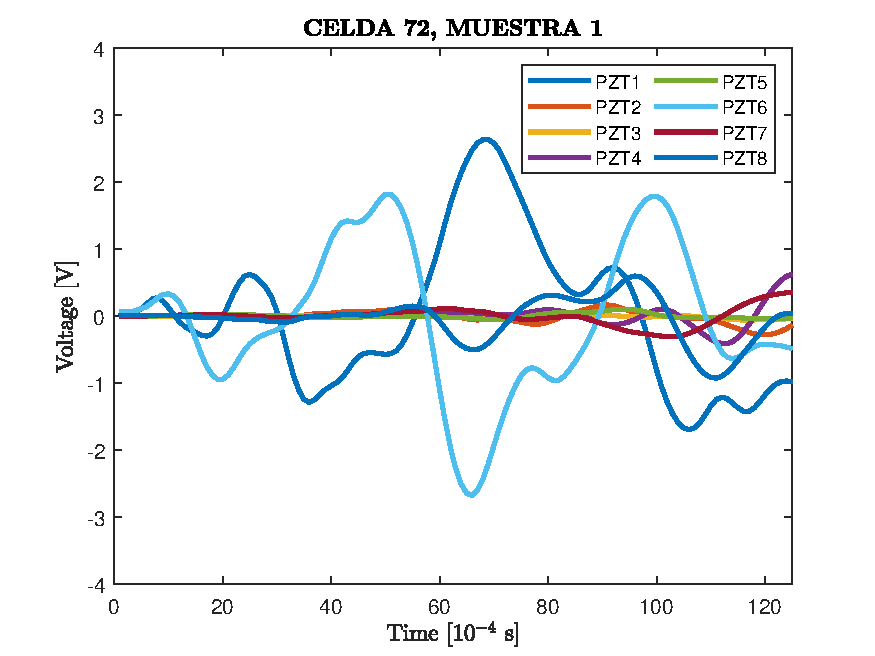
\includegraphics[width=75mm]{4/Fotos/Impacto_72_1.pdf}
    \label{}}
  \subfloat[Muestra 2 de impacto en celda 72]{
    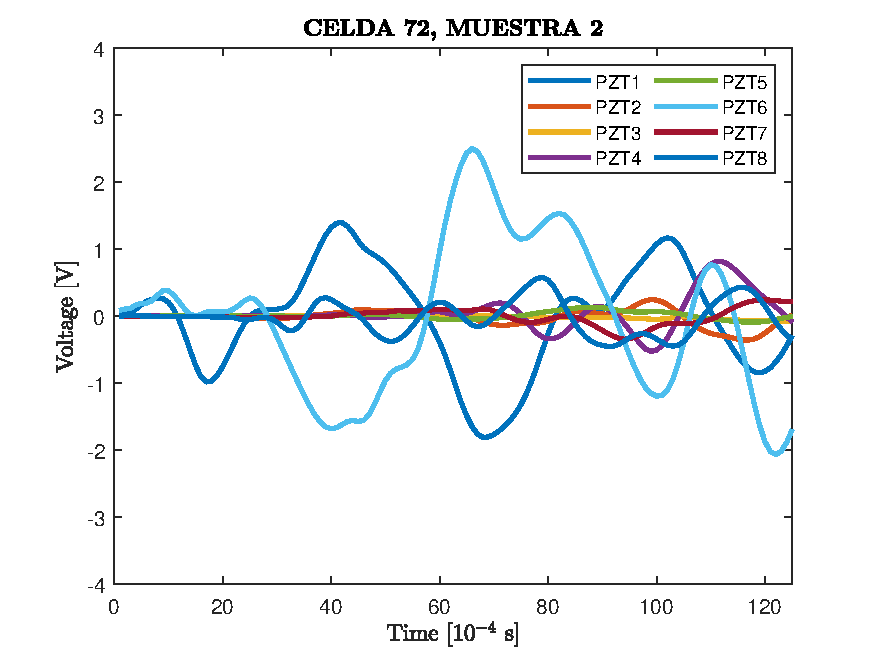
\includegraphics[width=75mm]{4/Fotos/Impacto_72_2.pdf}
    \label{}}
    \caption{Diferentes ejemplos de impactos}
    \label{fig:multiple_impactos}
\end{figure}


% -- -- %


\subsection{Modelo generativo de secuencias temporales}

¿Qué es un buen modelo generativo para datos de series temporales? El entorno temporal plantea un desafío único para el modelado generativo. Un modelo no sólo tiene la tarea de capturar las distribuciones de los rasgos dentro de cada punto temporal, sino que también debe capturar la dinámica potencialmente compleja de esas variables a lo largo del tiempo. Específicamente, en el modelado de datos secuenciales multivariable $x_{1:T} = (x1; ... ; x_T )$, también deseamos capturar con precisión la distribución condicional $p(x_t|x_{1:t1})$ de las transiciones temporales. 

Desde el 2014, gran parte del trabajo se ha centrado en mejorar la dinámica temporal de los modelos autorregresivos para la predicción de secuencias. Éstos abordan principalmente el problema de los errores de composición durante el muestreo de múltiples etapas, introduciendo diversas modificaciones en el momento de su formación para reflejar con mayor precisión las condiciones del tiempo de validación. Los modelos autorregresivos factorizan explícitamente la distribución de las secuencias en un producto de los condicionales $\Pi_t p(x_t|x_{1:t1})$. Sin embargo, aunque es útil en el contexto de la predicción, este enfoque es fundamentalmente determinista y no es verdaderamente generativo en el sentido de que se pueden tomar muestras aleatorias de nuevas secuencias a partir de ellas sin condicionamientos externos. Por otra parte, otra línea de trabajo se ha centrado en la aplicación directa del marco de las GANs a los datos secuenciales, principalmente mediante la instanciación de redes recurrentes para las funciones de generador y discriminador. Aunque es sencillo, el objetivo adversario busca modelar $p(x_{1:t1})$ directamente, sin apalancar el previo autorregresivo. Es importante, simplemente sumar la función de costes (loss) estándar de la GAN sobre las secuencias de vectores puede no ser suficiente para asegurar que la dinámica de la red capte eficientemente las dependencias escalonadas presentes en los datos de entrenamiento.\\

Las Redes Generativas Adversas de Series Temporales (TimeGAN) proponen un novedoso mecanismo para unir ambos hilos de la investigación, dando lugar a un modelo generativo explícitamente entrenado para preservar la dinámica temporal. TimeGAN crea, un marco natural para generar datos de series temporales realistas en varios dominios. 

\subsection{Arquitectura TimeGAN}

Como ya se ha mencionado al inicio de este capítulo, las GANs están constituidas principalmente por un generador y un discriminador. Sin embargo, la arquitectura de TimeGAN varía ligeramente de esta generalización con el objetivo de poder retener la dinámica de los datos temporales.

TimeGAN está formada por cuatro componentes: una función de integración, función de recuperación, generador de secuencia y discriminador de secuencia. 

La idea clave es que los componentes de autocodificación (los dos primeros) se entrenan conjuntamente con los componentes adversarios (los dos últimos), de modo que TimeGAN aprende simultáneamente a codificar características, generar representaciones e iterar a través del tiempo. La red de integración proporciona el espacio latente, la red adversaria opera dentro de este espacio y la dinámica latente de los datos reales y sintéticos se sincronizan a través de una pérdida supervisada (función de costes). Describimos cada uno a su vez.

\begin{itemize}
    \item[$\bullet$] \textbf{Funciones de integración y recuperación}
    
    Las funciones de integración y recuperación proporcionan asignaciones entre la característica y el espacio latente, lo que permite a la red adversaria aprender la dinámica temporal subyacente de los datos a través de representaciones de dimensiones más bajas.
    
    Sean $H_S$ y $H_{X}$ los espacios vectoriales latentes correspondientes a los espacios de las características $S$ y $X$. Entonces la función de integración $e : S \times \Pi_{t}X \rightarrow H_S \times \Pi_{t}H_X$ lleva las características estáticas y temporales a su estado latente $h_S, h_{1:t} = e(s,x_{1:T})$. $e$ se ha implementado mediante una RNN.
    
    \begin{equation}
        \textbf{h}_S = e_S(s), \qquad \qquad \textbf{h}_t = e_X (\textbf{h}_S, \textbf{h}_{t-1},\textbf{x}_t)
    \end{equation}
    
    donde $e_S : S \rightarrow H_S$ es ina red integradora para variables estáticas, y $e_X : H_S \times H_X \times X \rightarrow H_X$ una red recurrente integradora para características temporales. En la dirección opuesta, la función recuperadora $r : H_S \times \Pi_{t}H_X \rightarrow S \times \Pi_{t}X$ coge las características latentes y las devuelve al espacio de características $\~s, \~x_{1:T} = r(\textbf{h}_S, \textbf{h}_{1:T})$. Aquí se implementa $r$ usando una red \textit{feedforward} en cada paso
    
    \begin{equation}
        \~s = r_{S}(\textbf{h}_s), \qquad  \~x_t = r_{X}(\textbf{h}_t)
    \end{equation}
    
    donde $r_S : H_S \rightarrow S$ y $r_X : H_X \rightarrow X$ son redes de recuperación para las integraciones estáticas y temporales.
    
    \item[$\bullet$] \textbf{Generador y discriminador de secuencias}
    
    En ved de generar datos sintéticos directamente en el espacio de características, el generador primero crea su salida en el espacio de integración. Sean $Z_S$ y $Z_{X}$ los espacios vectoriales sobre los que sabemos que las distribuciones están definidas y de donde se extraen los vectores aleatorios como entrada para generar $H_S$ y $H_{X}$. Entonces la función de generación $g : Z_S \times \Pi_{t}Z_X \rightarrow H_S \times \Pi_{t}H_X$ lleva una pareja de vectores aleatorios estáticos y temporaes al espacio latente sintético $\^h_S, \^h_{1:T} = g(\textbf{z}_S, \textbf{z}_{1:T})$. Se implementa g con una RNN.
    
    \begin{equation}
        \textbf{\^h}_S = g_S(\textbf{z}_S), \qquad \qquad \textbf{\^h}_t = g_X (\textbf{\^h}_S, \textbf{\^h}_{t-1},\textbf{z}_t)
    \end{equation}
    
    donde $g_S : Z_S \rightarrow H_S$ es una red generadora de características estáticas y $g_X : H_S \times H_X \times Z_X \rightarrow H_X$ es un generador recurrente para características temporales. Vectores aleatorios $\textbf{z}_S$ pueden ser muestreados desde una distribución cualquiera y $\textbf{z}_t$ sigue un proceso estocástico. Aquí se usa una distribución y un proceso Winer respectivamente. Finalmente el discriminador también opera en es espacio integrado. La función discriminatoria $d : H_S \times \Pi_t H_X \rightarrow [0,1] \times \Pi_t[0,1]$ recibe las características temporales y estáticas, devolviendo la clasificación $\~y_S, \~y_{1:T} = d(\textbf{\~h}_S), \textbf{\~h}_{1:T}$. La notación $\textbf{\~h}$ refiera a datos reales ($h$) como sintéticos ($\^h$) en el espacio vectorial de integración, al igual que $\textbf{\~y}$ indica clasificación real ($y$) como sintética ($\^y$). Aquí se implementa d a partir de una RNN bidimensional con una capa \textit{feedforward} en la salida
    
    \begin{equation}
        \textbf{\~y}_S = d_S(\textbf{\~h}_S), \qquad \qquad \textbf{\~y}_t = d_X (\cev{\textbf{u}}_t, \vec{\textbf{u}}_{t})
    \end{equation}
    
    donde $\cev{\textbf{u}}_{t} = \cev{c_X}(\vec{\textbf{\~h}_S},\vec{\textbf{\~h}}_t,\vec{\textbf{u}}_{t-1})$ y $\vec{\textbf{u}}_{t} = \vec{c_X}(\vec{\textbf{\~h}_S},\vec{\textbf{\~h}}_t,\cev{\textbf{u}}_{t+1})$ respectivamente denotan las secuencias hacia adelante y atrás de los \textit{hidden states}, $\vec{c}_X$ y $\cev{c}_X$ son finciones recurrentes y  $d_S$, $d_X$ son las funciones de clasificación de la última capa.
\end{itemize}

El diagrama de bloques del funcionamiento de TimeGAN se puede ver en la Figura \ref{fig:TimeGAN}\\

\begin{figure}[h!]
    \centering
    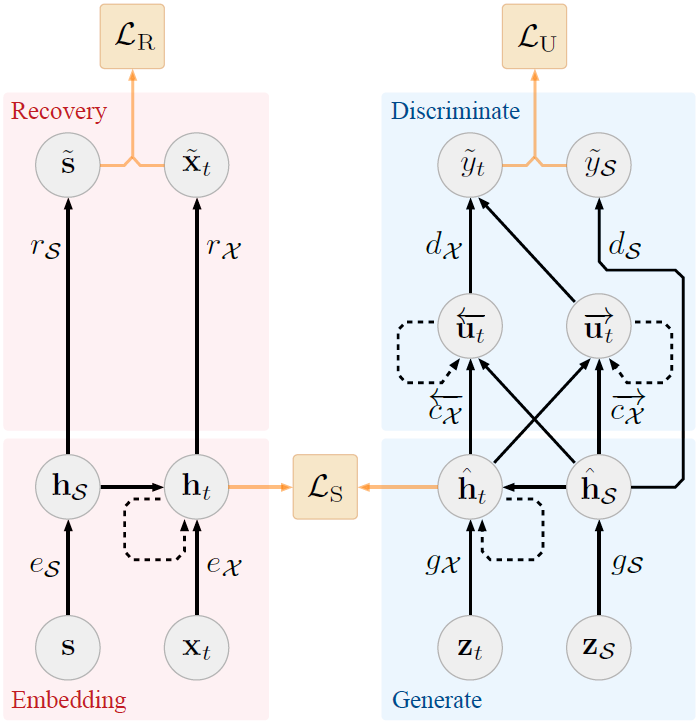
\includegraphics[width=125mm, angle=0]{4/Fotos/TimeGAN.png}
    \captionsetup{justification=centering,margin=1.25cm}
    \caption{Diagrama de bloques del funcionamiento de TimeGAN}
    \label{fig:TimeGAN}
\end{figure}

Todo lo comentado sobre TimeGAN en este trabajo ha sido extraído de \cite{TimeGAN}. Aquí se puede encontrar tanto el paper de su publicación como el código necesario para la implementación de esta red.


% -- -- %


\subsection{Resultados de la generación de impactos con TimeGAN}

Antes de comenzar con el proceso de generación de impactos es necesario definir una serie de parámetros de arquitectura y del proceso de entrenamiento.

\begin{itemize}
    \item[$\bullet$] Tipo de capa recurrente: GRU
    \item[$\bullet$] Número de neuronas en las capas ocultas: 64
    \item[$\bullet$] Número de épocas en el entrenamiento: 400
\end{itemize}

Con los parámetros ya definidos se puede comenzar el proceso. Es importante tener en cuenta que se van a generar los impactos de forma individual e independiente. Esto quiere decir que se introducirán a la red todos los impactos reales de, por ejemplo, la celda 11 y una vez que se haya entrenado la TimeGAN se generarán 1500 impactos sintéticos. Después se borrará todo el aprendizaje que la red haya generado y se introducirán los impactos de la siguiente celda y volverá a repetirse el ciclo. \\

En la Figura \ref{fig:multiple_impactos_S} se puede ver varios impactos sintéticos que coinciden con las celdas elegidas en la Figura \ref{fig:multiple_impactos}. Si se comparan visualmente se podrían confundir con un impacto real sin ninguna dura.

\begin{figure}[h!]
 \centering
  \subfloat[Muestra 1 de impacto en celda 11]{
    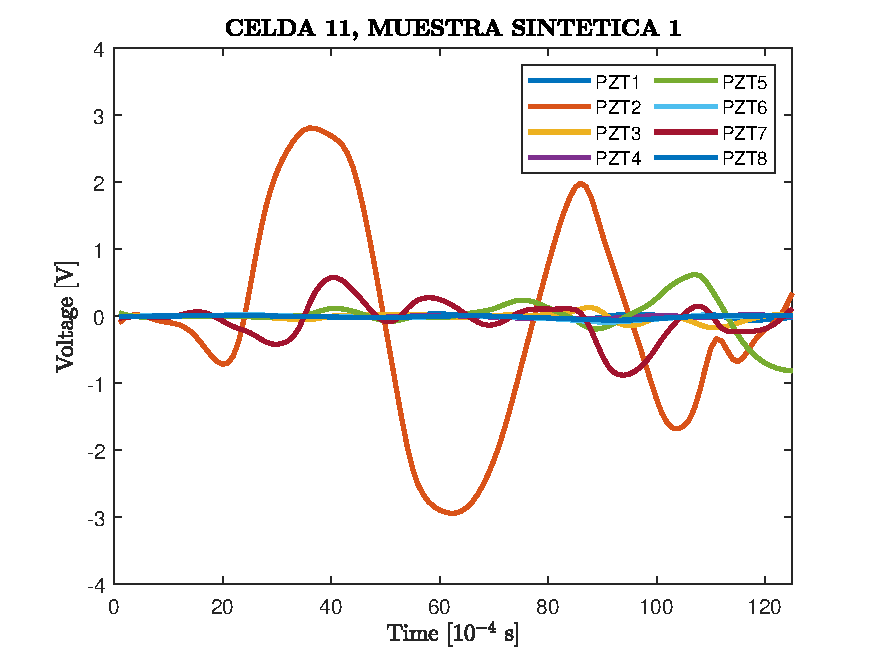
\includegraphics[width=75mm]{4/Fotos/Impacto_11_1_S.pdf}
    \label{fig:celda_11_1_S}}
  \subfloat[Muestra 2 de impacto en celda 11]{
    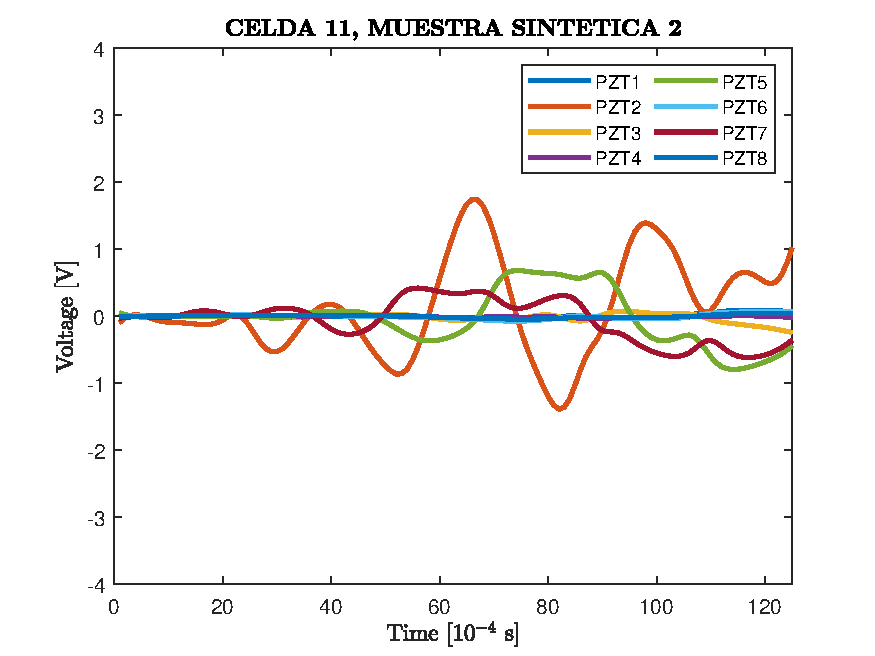
\includegraphics[width=75mm]{4/Fotos/Impacto_11_2_S.pdf}
    \label{fig:celda_11_2_S}}
    \label{Esto solo esta aqui para separar en dos bloques}
  \subfloat[Muestra 1 de impacto en celda 72]{
    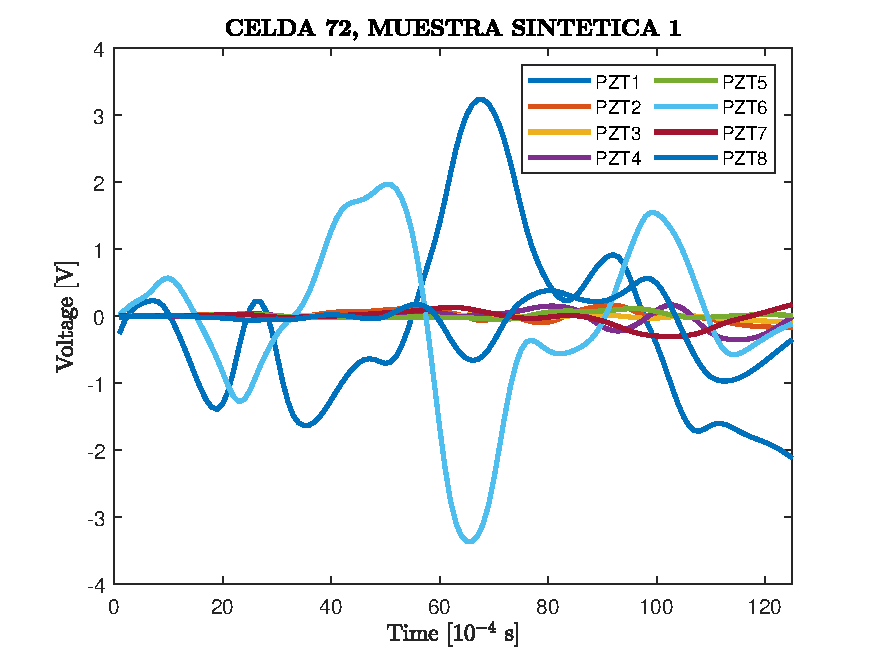
\includegraphics[width=75mm]{4/Fotos/Impacto_72_1_S.pdf}
    \label{}}
  \subfloat[Muestra 2 de impacto en celda 72]{
    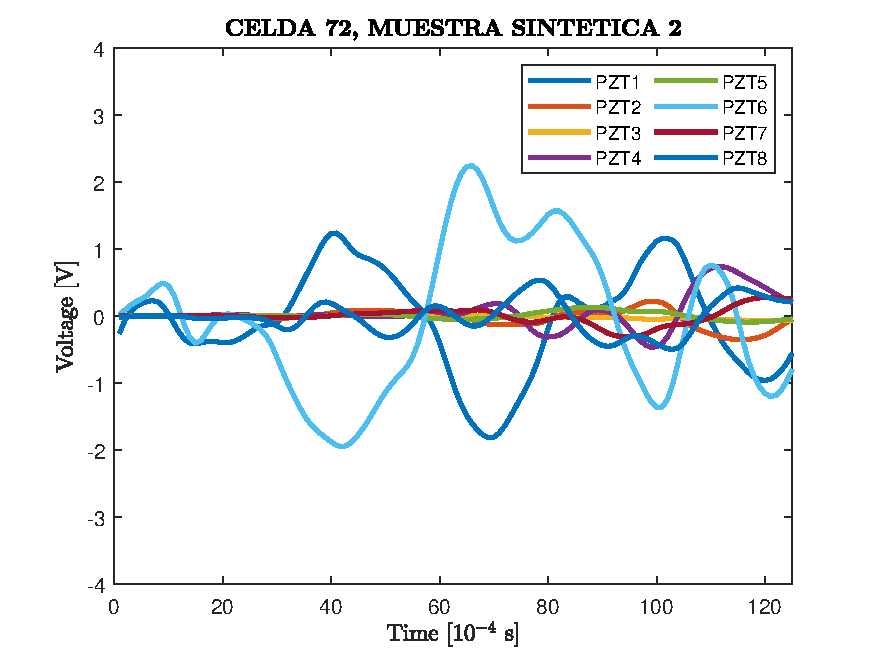
\includegraphics[width=75mm]{4/Fotos/Impacto_72_2_S.pdf}
    \label{}}
    \caption{Diferentes ejemplos de impactos generados sintéticamente con TimeGAN}
    \label{fig:multiple_impactos_S}
\end{figure}

Pero para tener un nivel alto de confianza en que los nuevos datos que se han generado sintéticamente son ciertamente equivalentes a los impactos reales se ha decidido utilizar el algoritmo t-SNE de visualización.

En el capítulo 3, este algoritmo demostró que los daños similares se agrupaban en grupos o \textit{clusters} independientes, por lo tanto, para poder considerar que los impactos reales y generados son similares dentro de una celda y diferentes al resto de celdas lo que se espera al ejecutar el algoritmo es lo siguiente:

\begin{itemize}
    \item[$\bullet$] cada celda esté en un cluster independiente
    \item[$\bullet$] los impactos reales y sintéticos de una misma celda estén distribuidos de forma uniforme en el cluster correspondiente
\end{itemize}

\begin{figure}[H]
    \centering
    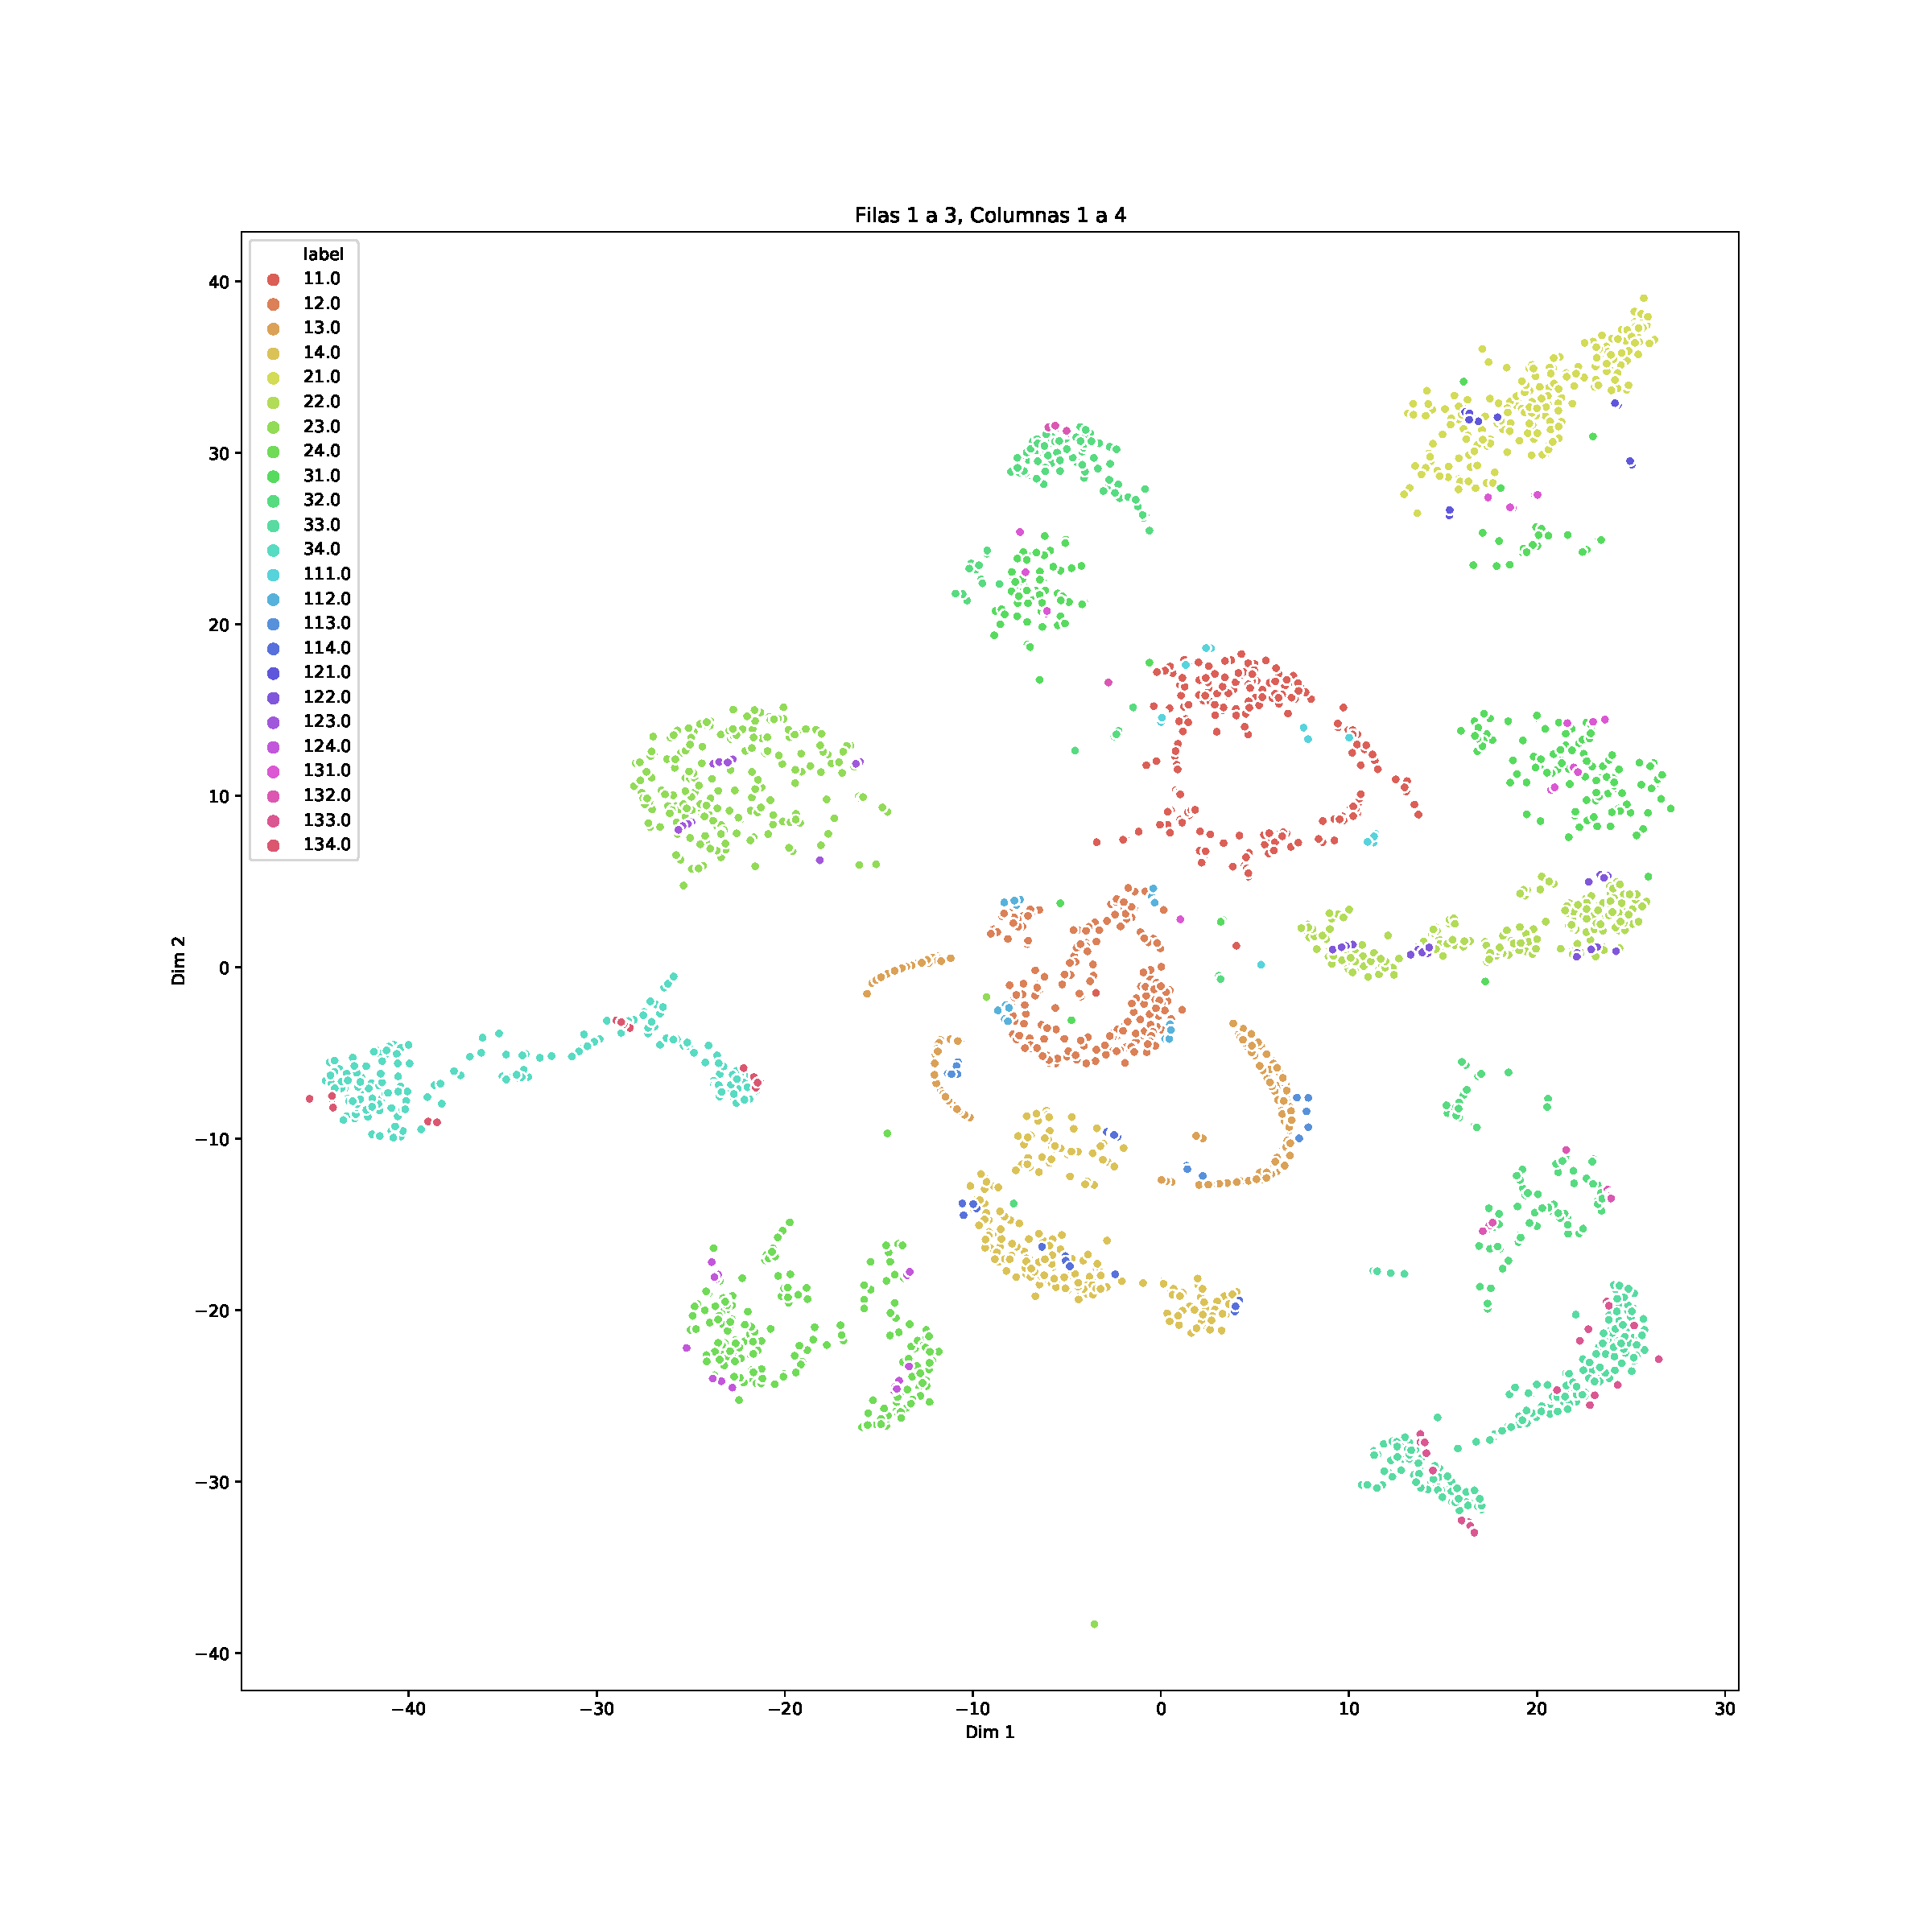
\includegraphics[width=110mm, angle=0]{4/Fotos/tsne_TimeGAN_13-14.pdf}
    \captionsetup{justification=centering,margin=1.25cm}
    \caption{t-SNE de las celdas 11, 12, 13, 14, 21, 22, 23, 24, 31, 32, 33, 34}
    \label{fig:13-14}
\end{figure}

\begin{figure}[H]
    \centering
    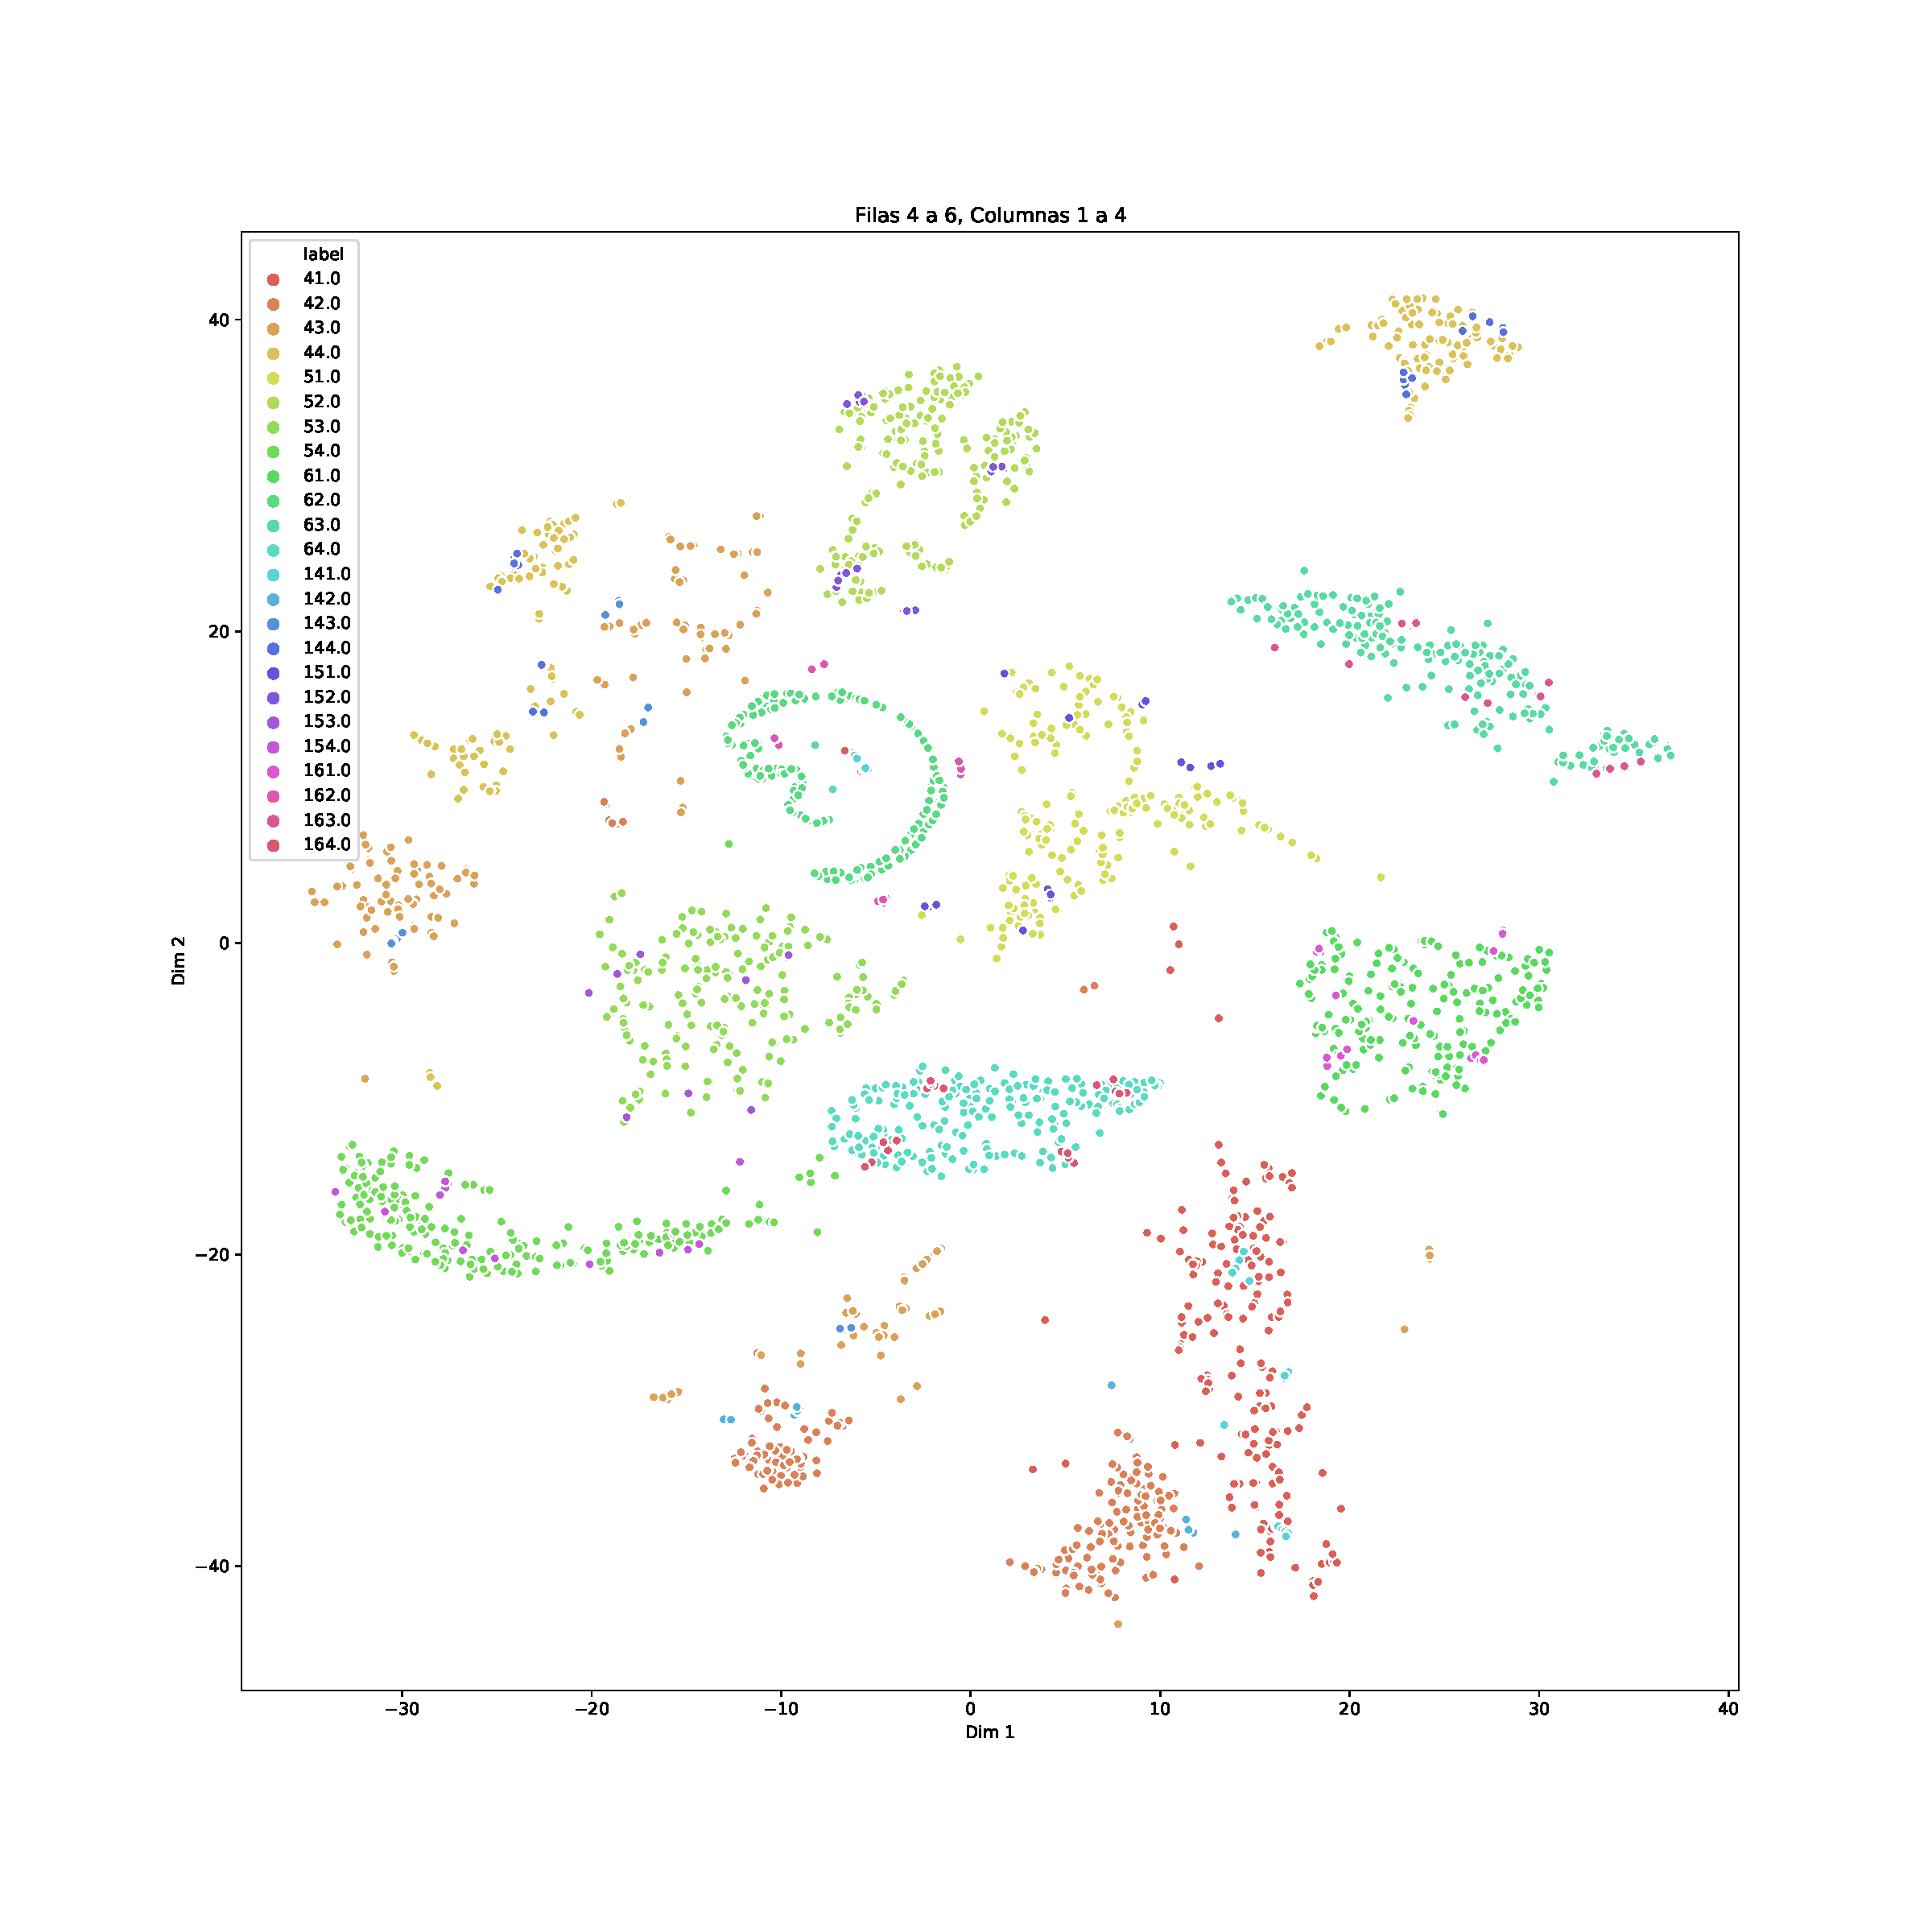
\includegraphics[width=110mm, angle=0]{4/Fotos/tsne_TimeGAN_46-14.pdf}
    \captionsetup{justification=centering,margin=1.25cm}
    \caption{t-SNE de las celdas 41, 42, 43, 44, 51, 52, 53, 54, 61, 62, 63, 64}
    \label{fig:46-14}
\end{figure}

\begin{figure}[H]
    \centering
    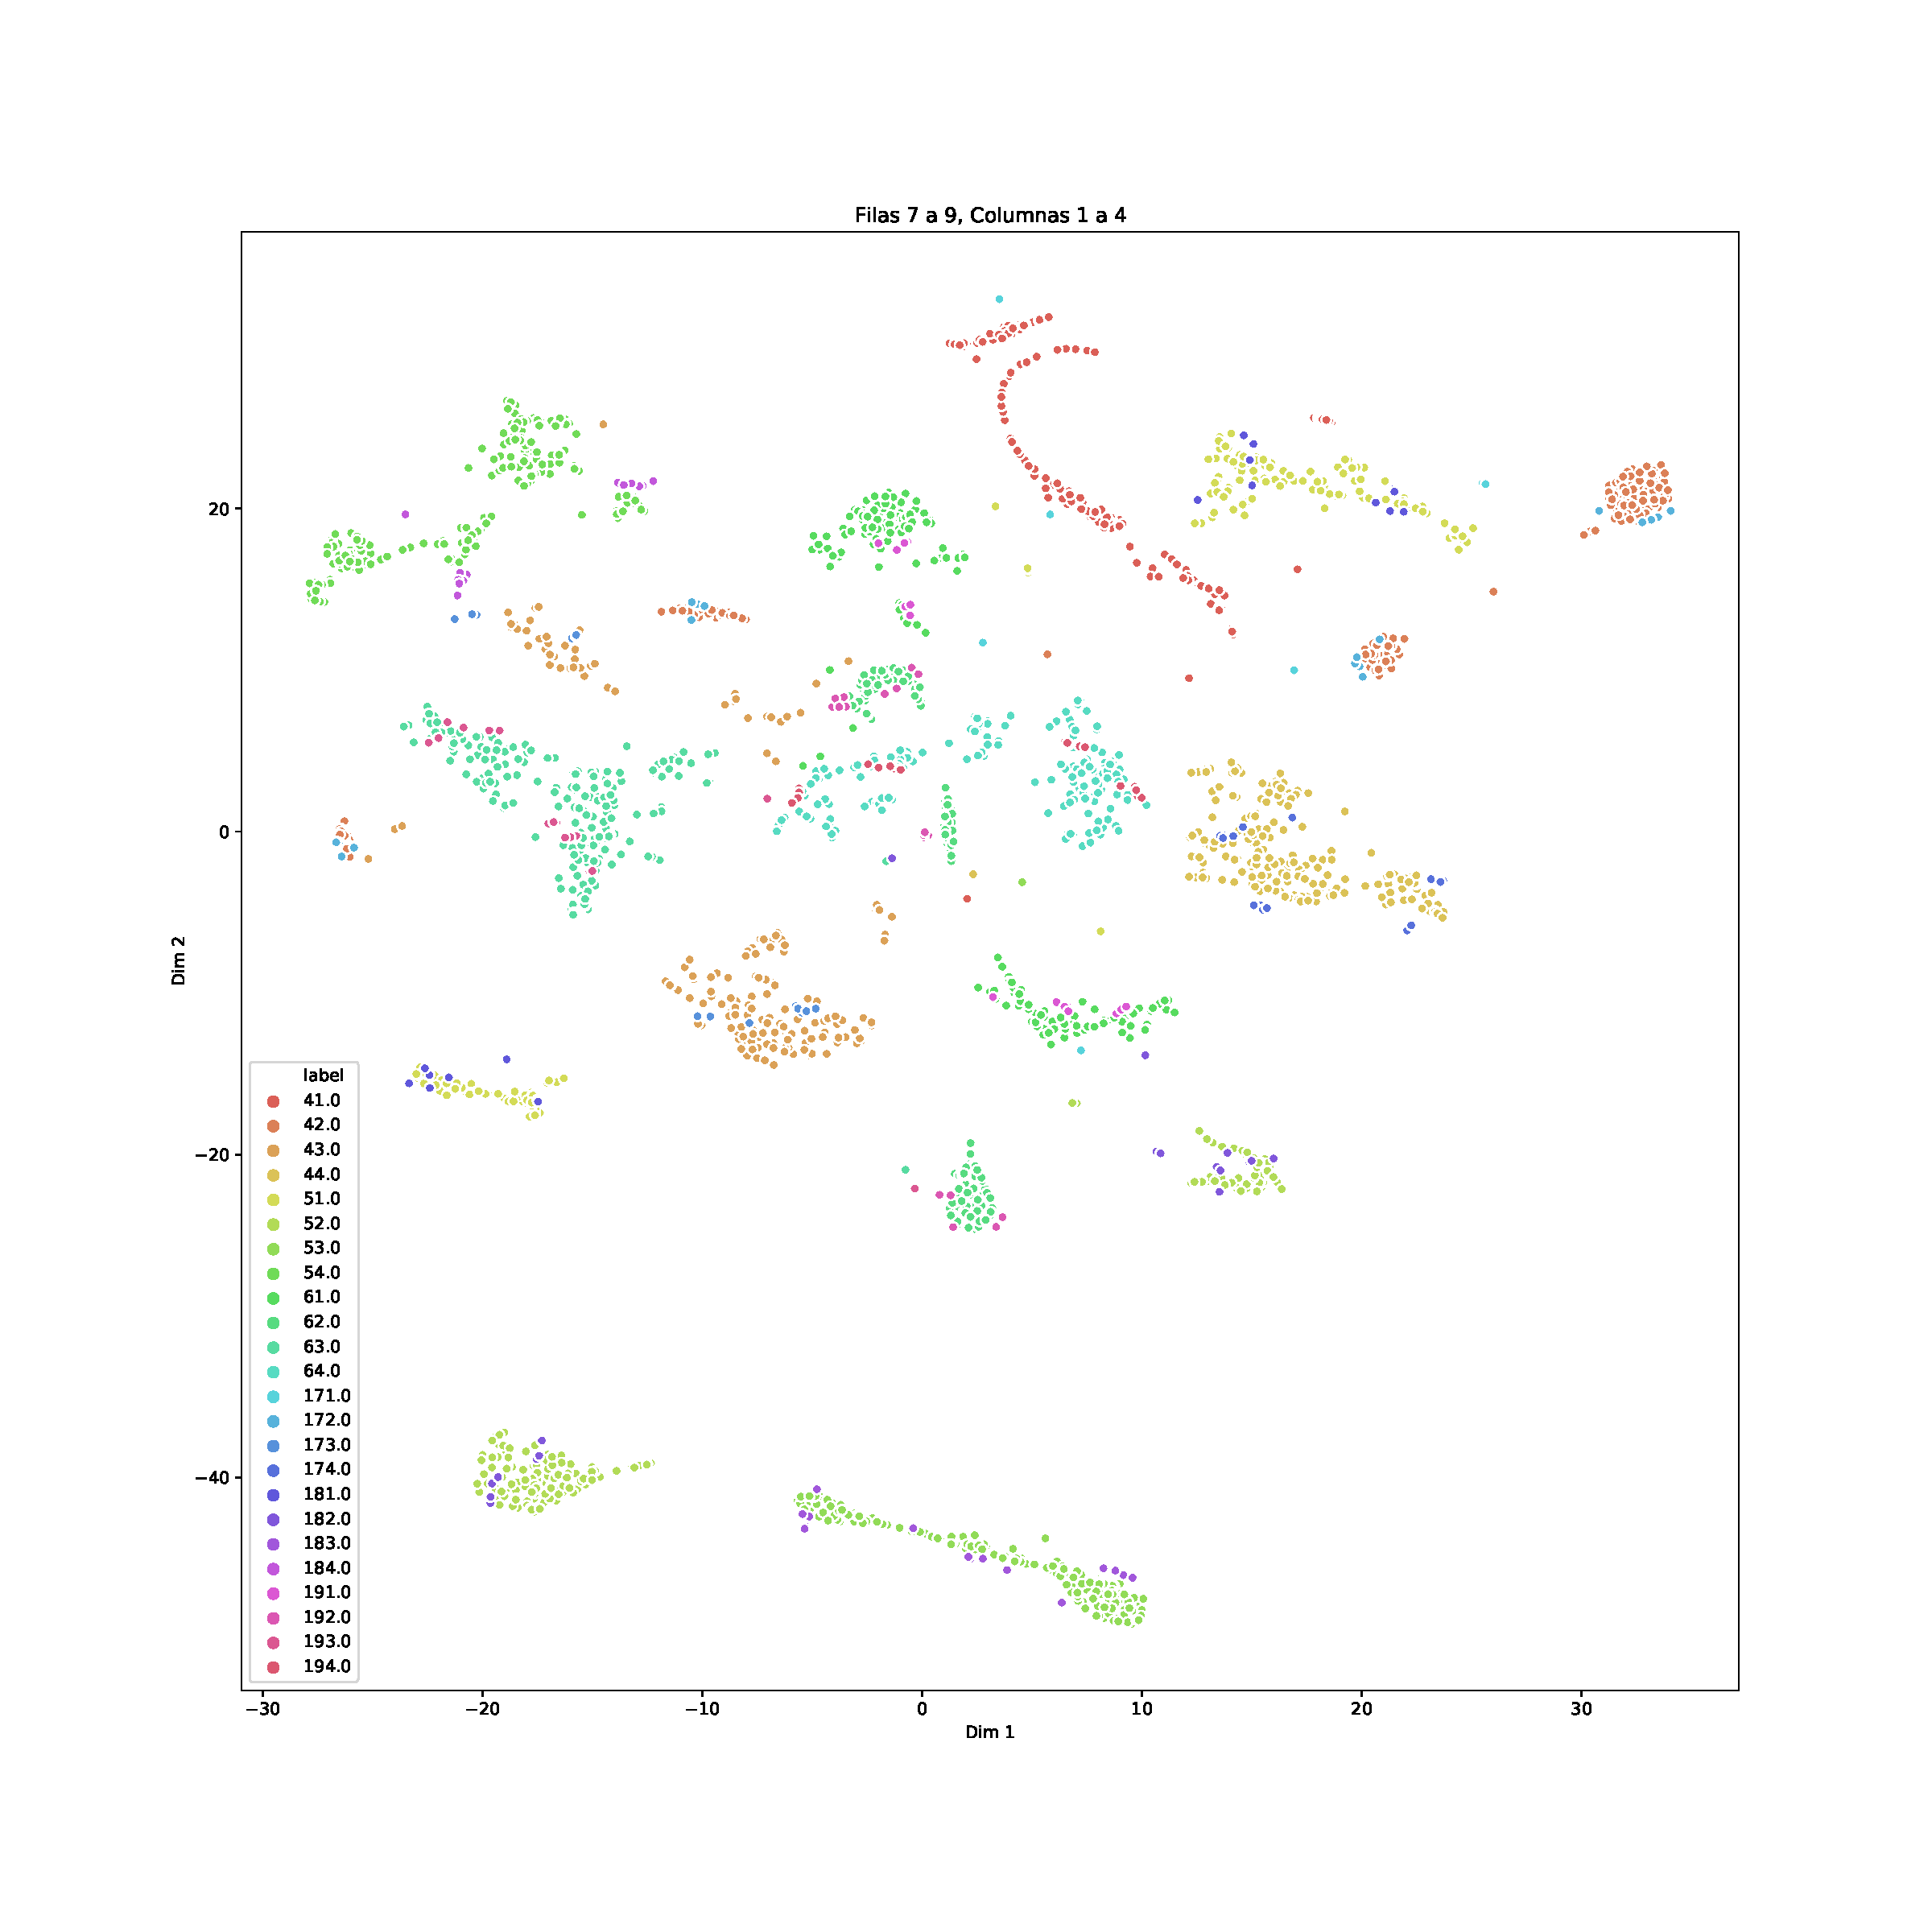
\includegraphics[width=110mm, angle=0]{4/Fotos/tsne_TimeGAN_79-14.pdf}
    \captionsetup{justification=centering,margin=1.25cm}
    \caption{t-SNE de las celdas 71, 72, 73, 74, 81, 82, 83, 84, 91, 92, 93, 94}
    \label{fig:79-14}
\end{figure}

\begin{figure}[H]
    \centering
    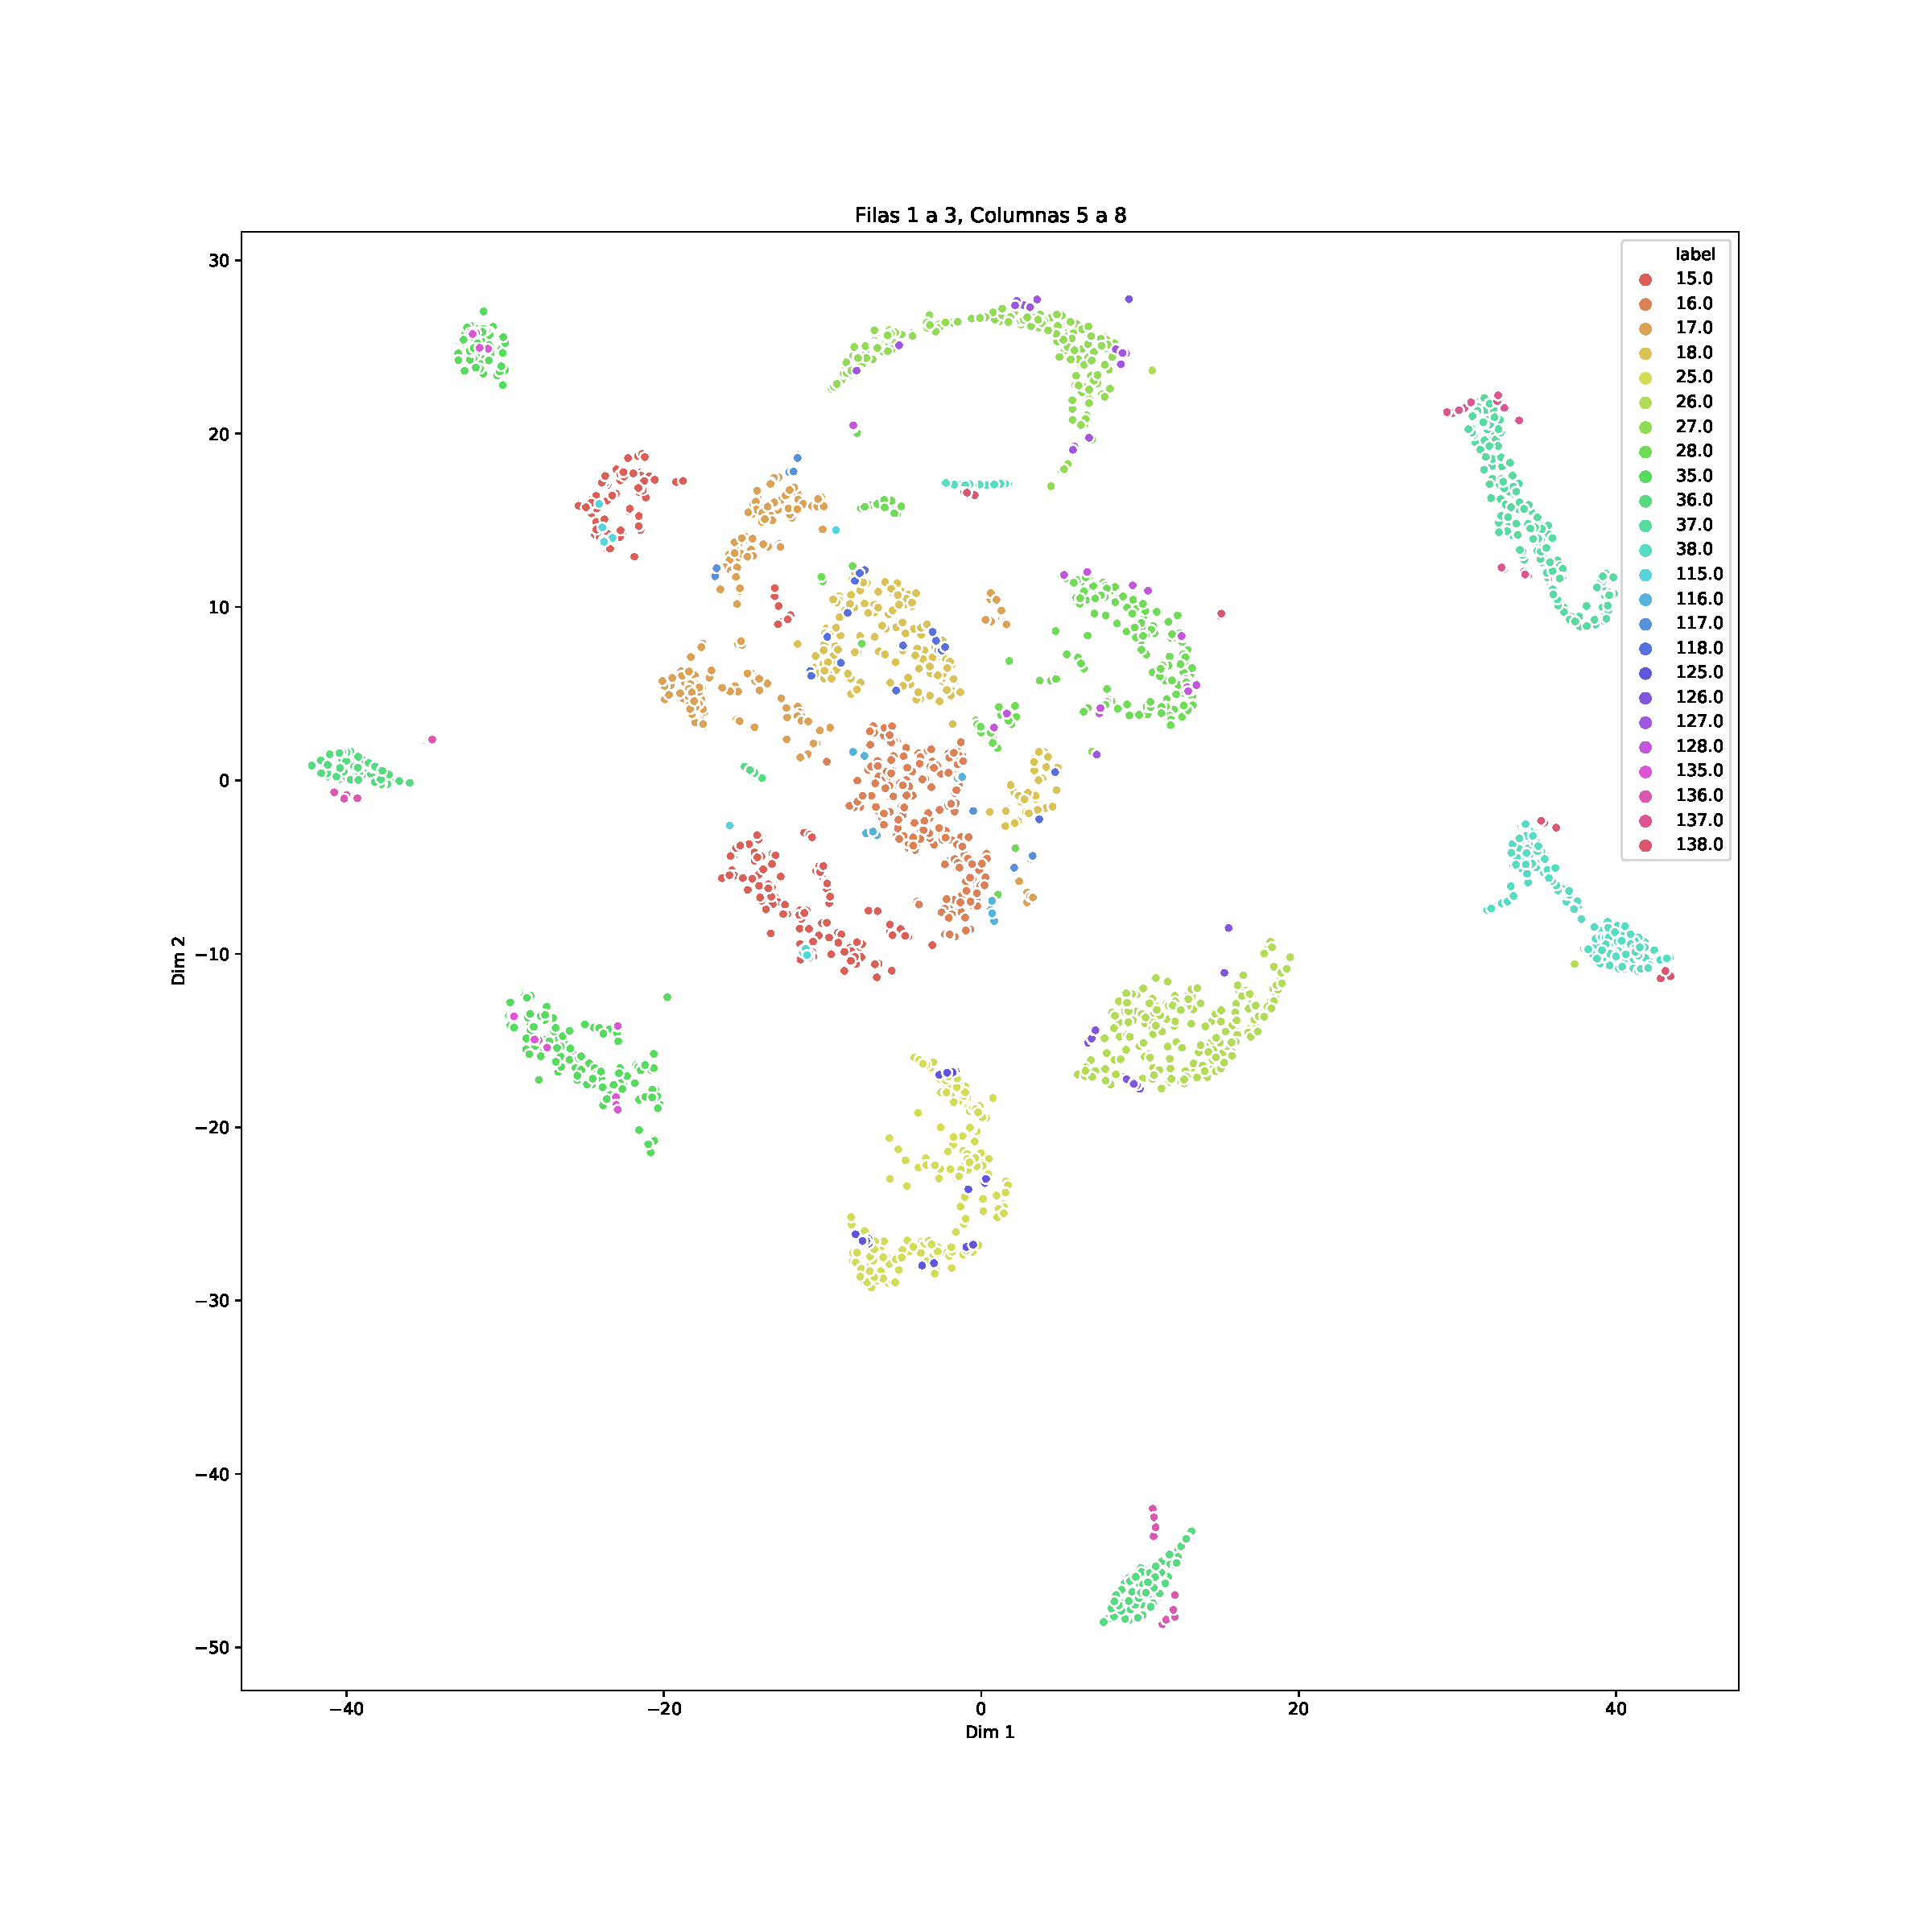
\includegraphics[width=110mm, angle=0]{4/Fotos/tsne_TimeGAN_13-58.pdf}
    \captionsetup{justification=centering,margin=1.25cm}
    \caption{t-SNE de las celdas 15, 16, 17, 18, 25, 26, 27, 28, 35, 36, 37, 38}
    \label{fig:13-58}
\end{figure}

\begin{figure}[H]
    \centering
    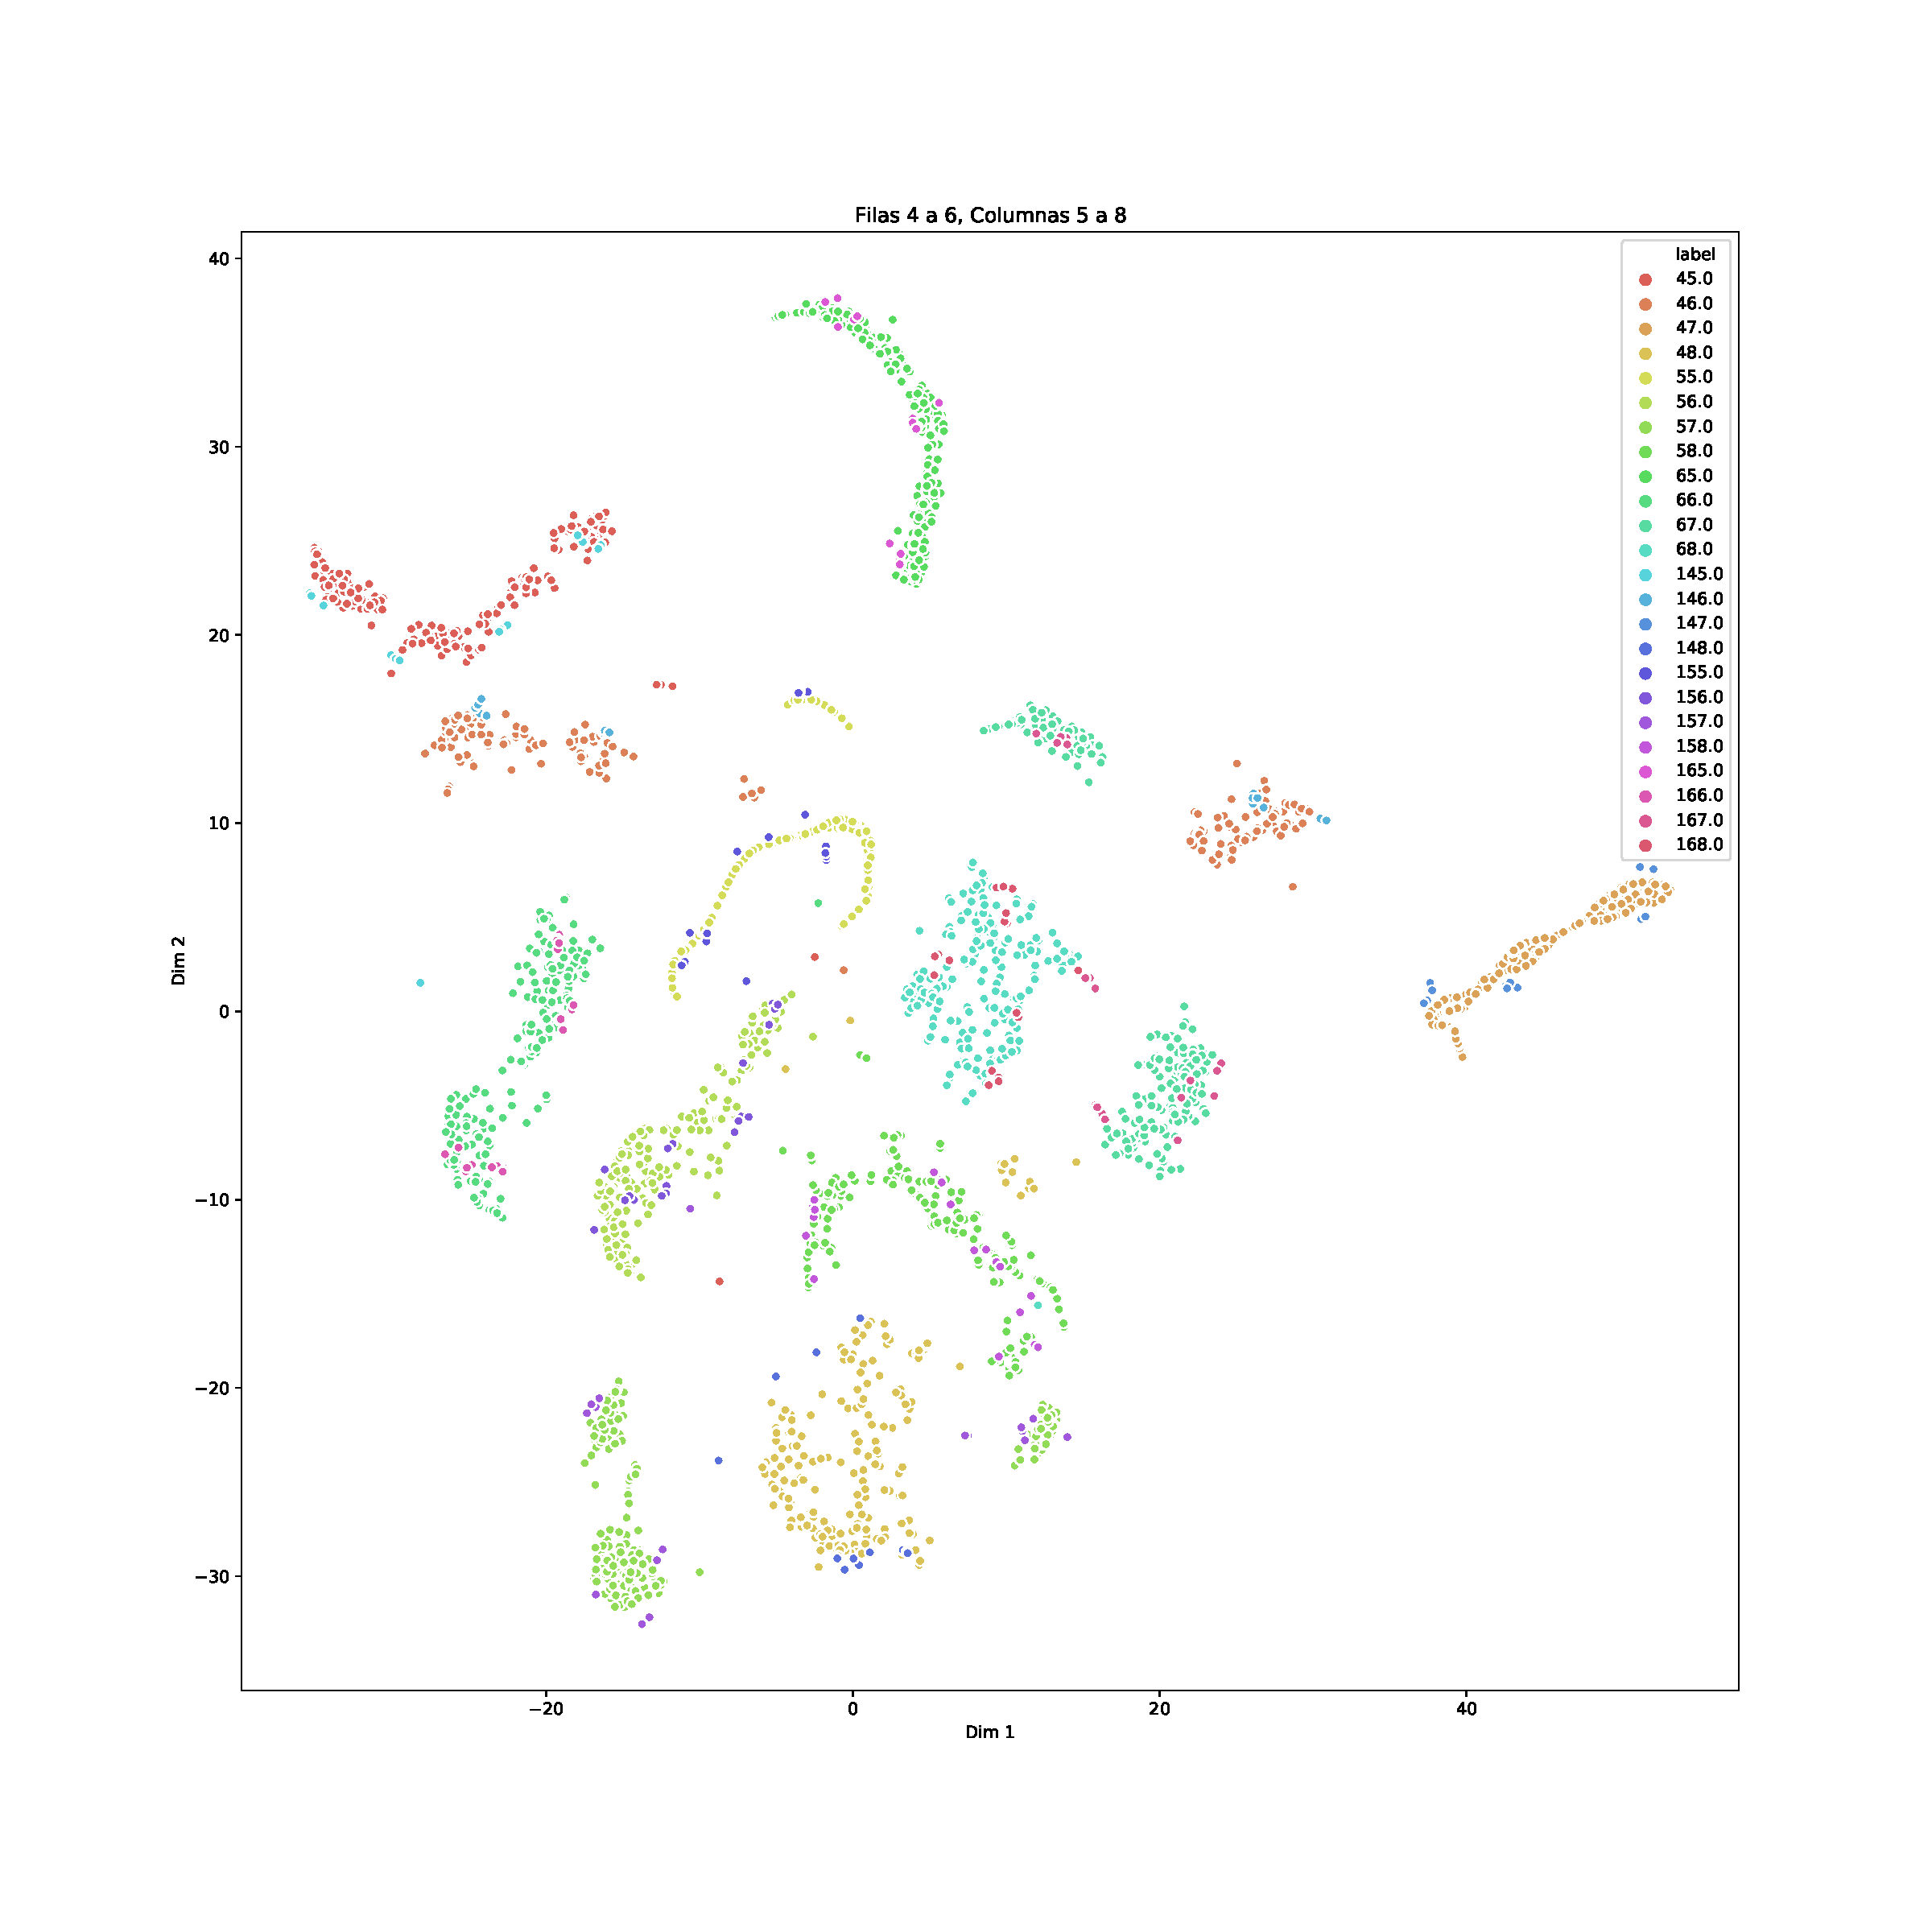
\includegraphics[width=110mm, angle=0]{4/Fotos/tsne_TimeGAN_46-58.pdf}
    \captionsetup{justification=centering,margin=1.25cm}
    \caption{t-SNE de las celdas 45, 46, 47, 48, 55, 56, 57, 58, 65, 66, 67, 68}
    \label{fig:46-58}
\end{figure}

\begin{figure}[H]
    \centering
    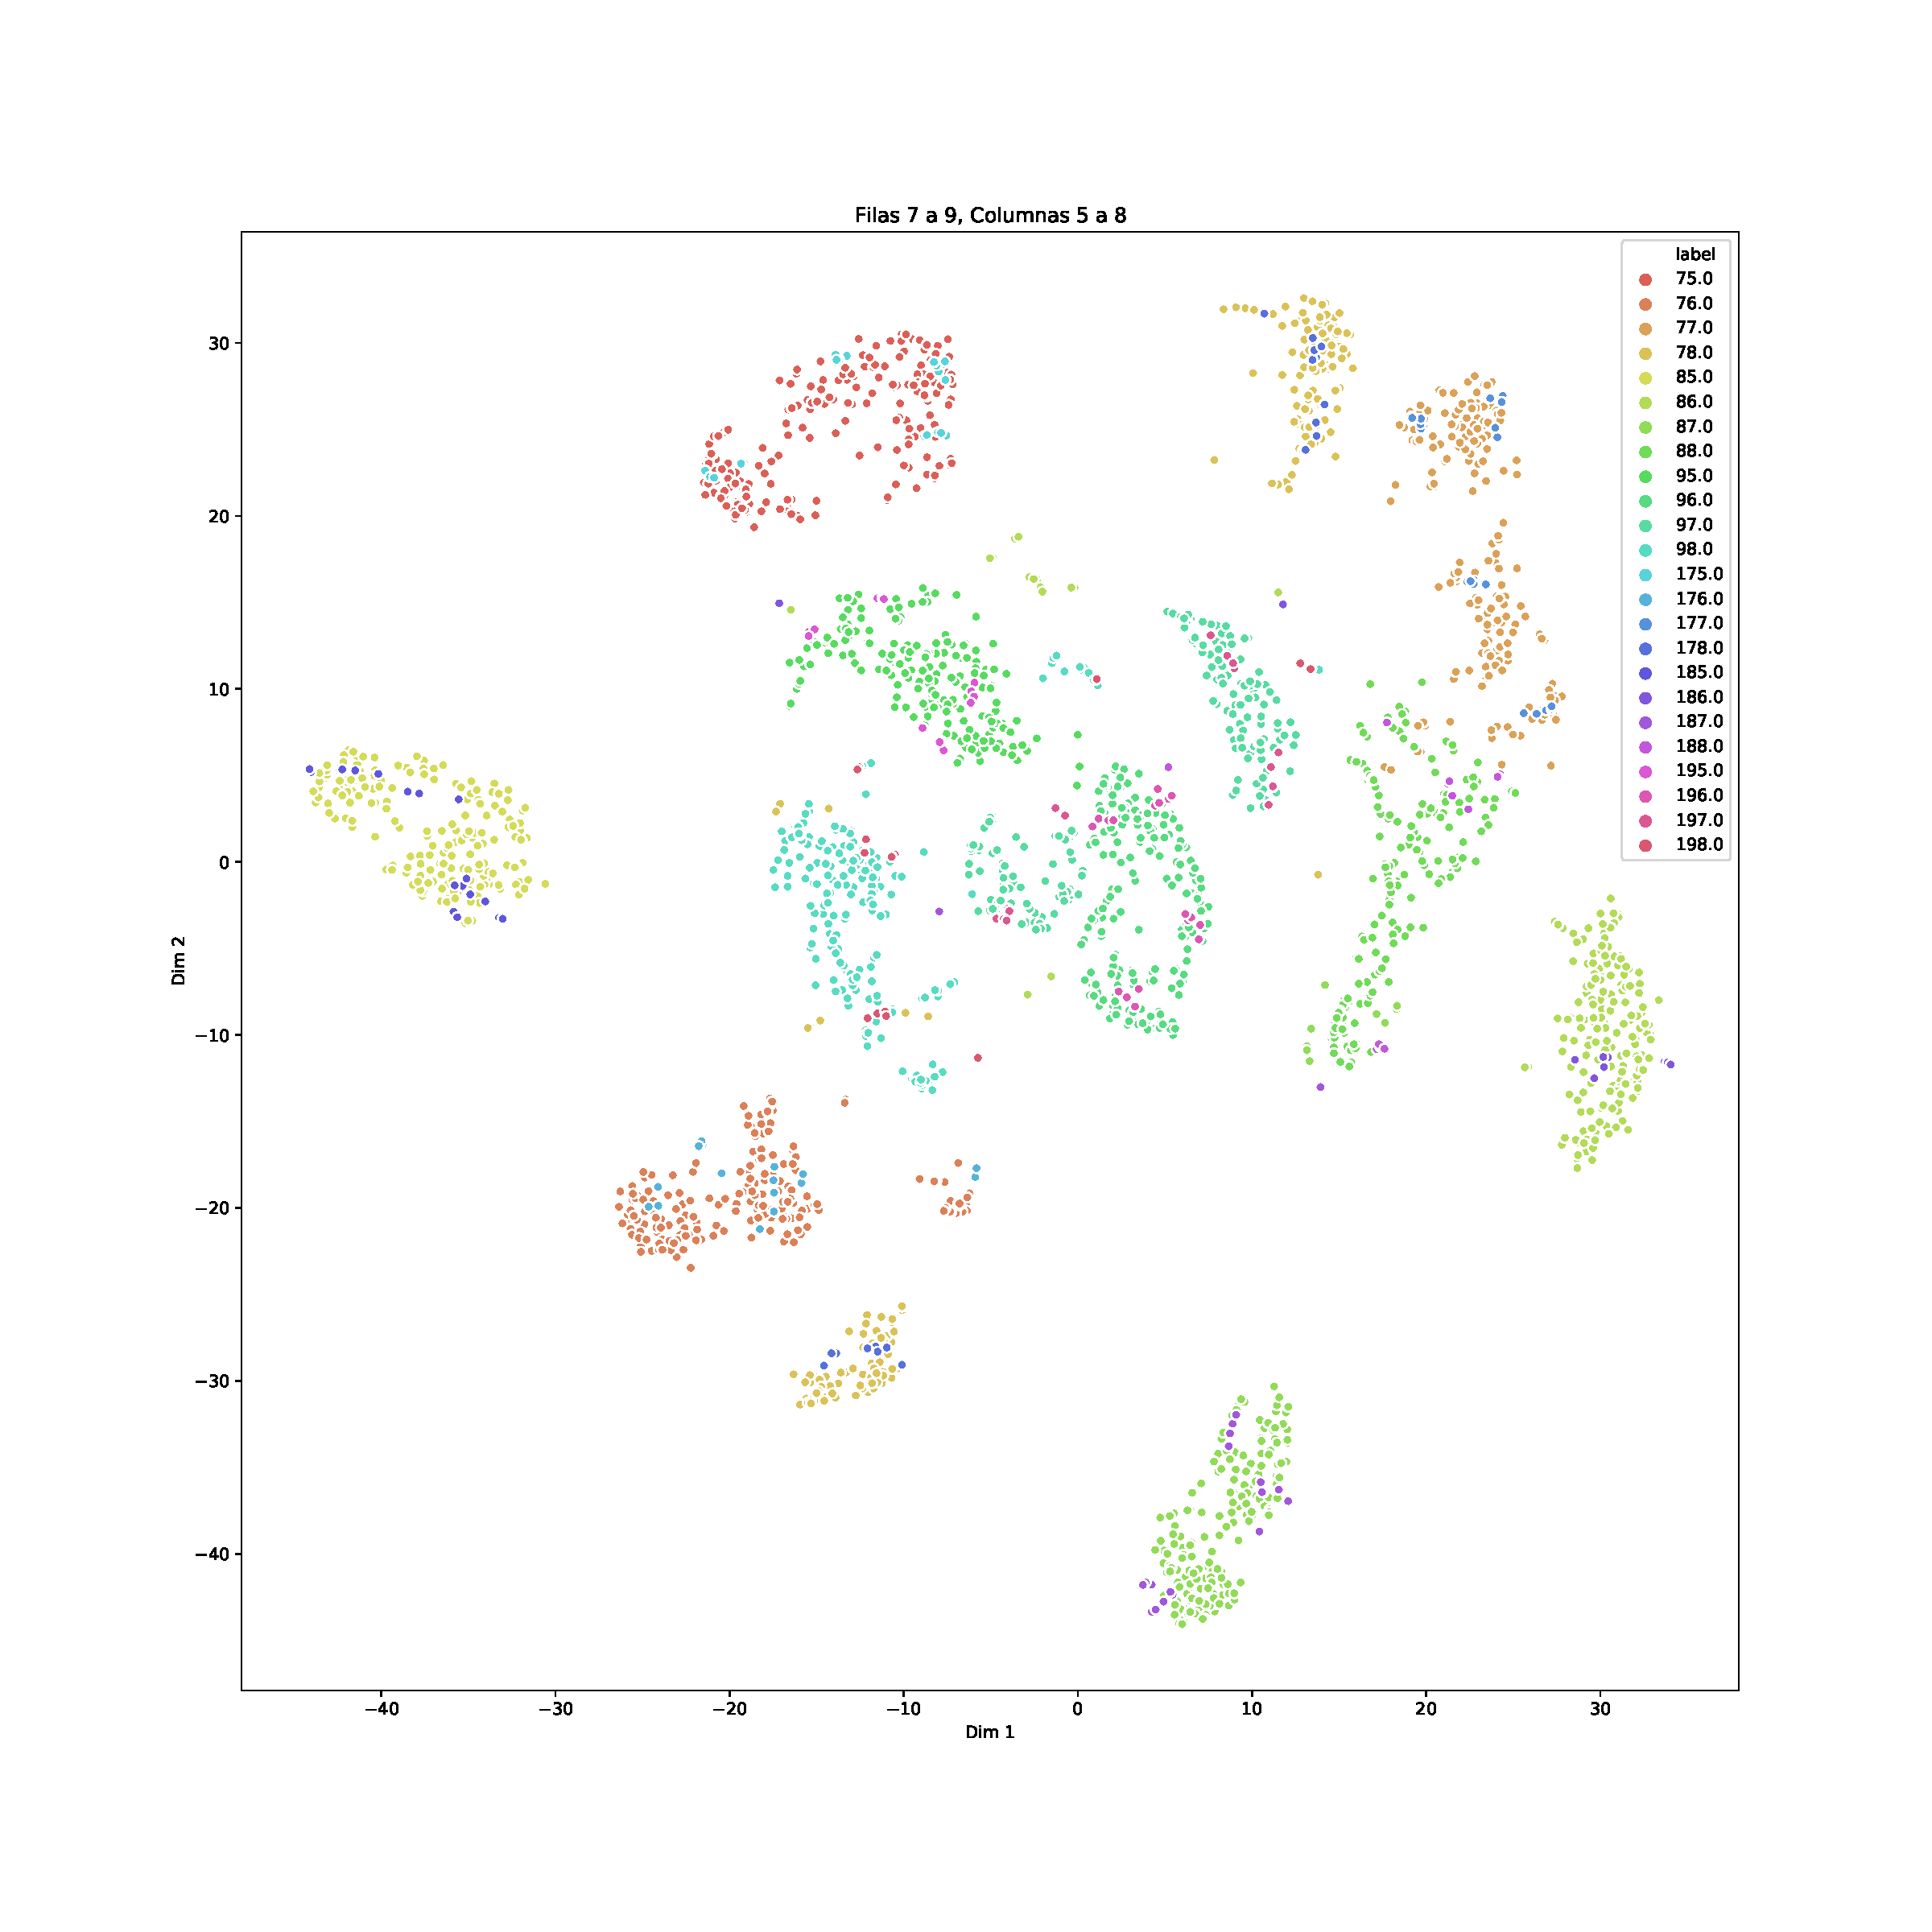
\includegraphics[width=110mm, angle=0]{4/Fotos/tsne_TimeGAN_79-58.pdf}
    \captionsetup{justification=centering,margin=1.25cm}
    \caption{t-SNE de las celdas 75, 76, 77, 78, 85, 86, 87, 88, 95, 96, 97, 98}
    \label{fig:79-58}
\end{figure}

De la Figura \ref{fig:13-14} a \ref{fig:79-58} se puede ver la representación de los impactos en las diferentes celdas. Al haber 72 celdas en total, se ha decidido realizar la visualización en grupos de 3x4. De este modo se puede entender de forma más sencilla las relaciones entre datos sintéticos y reales al haber menos puntos por figura.

En la leyendas hay dos tipos de datos diferentes, xx y 1xx. Los xx corresponden a los impactos sintéticos y los 1xx son sus homólogos reales.\\

En la Figura \ref{fig:13-14} se puede ver con claridad que los puntos correspondientes a la celda 34 están distribuidos entre dos agrupaciones pequeñas de los puntos 134. Esto quiere decir que los impactos sintéticos son similares a los reales y, a su vez, diferentes al resto de impactos.

Con este resultado se puede considerar que TimeGAN ha generado unos impactos similares a los reales y que se pueden utilizar para alimentar a una red clasificadora.

\clearpage


%  -----------------------------------------  %


\section{Caracterización de la posición}

\subsection{Arquitectura del clasificador}

Falta preparar el modelo de arquitectura para que se vea bien.


%  --  --  %


\subsection{Resultados}

Como la cantidad de impactos reales que se tienen es muy reducida, se ha decidido entrenar al clasificador únicamente con los impactos generados sintéticamente. Esto permite comprobar también el funcionamiento de un clasificador cuando los datos de entrenamiento y validación tienen cierta dispersión.\\

\begin{figure}[H]
    \centering
    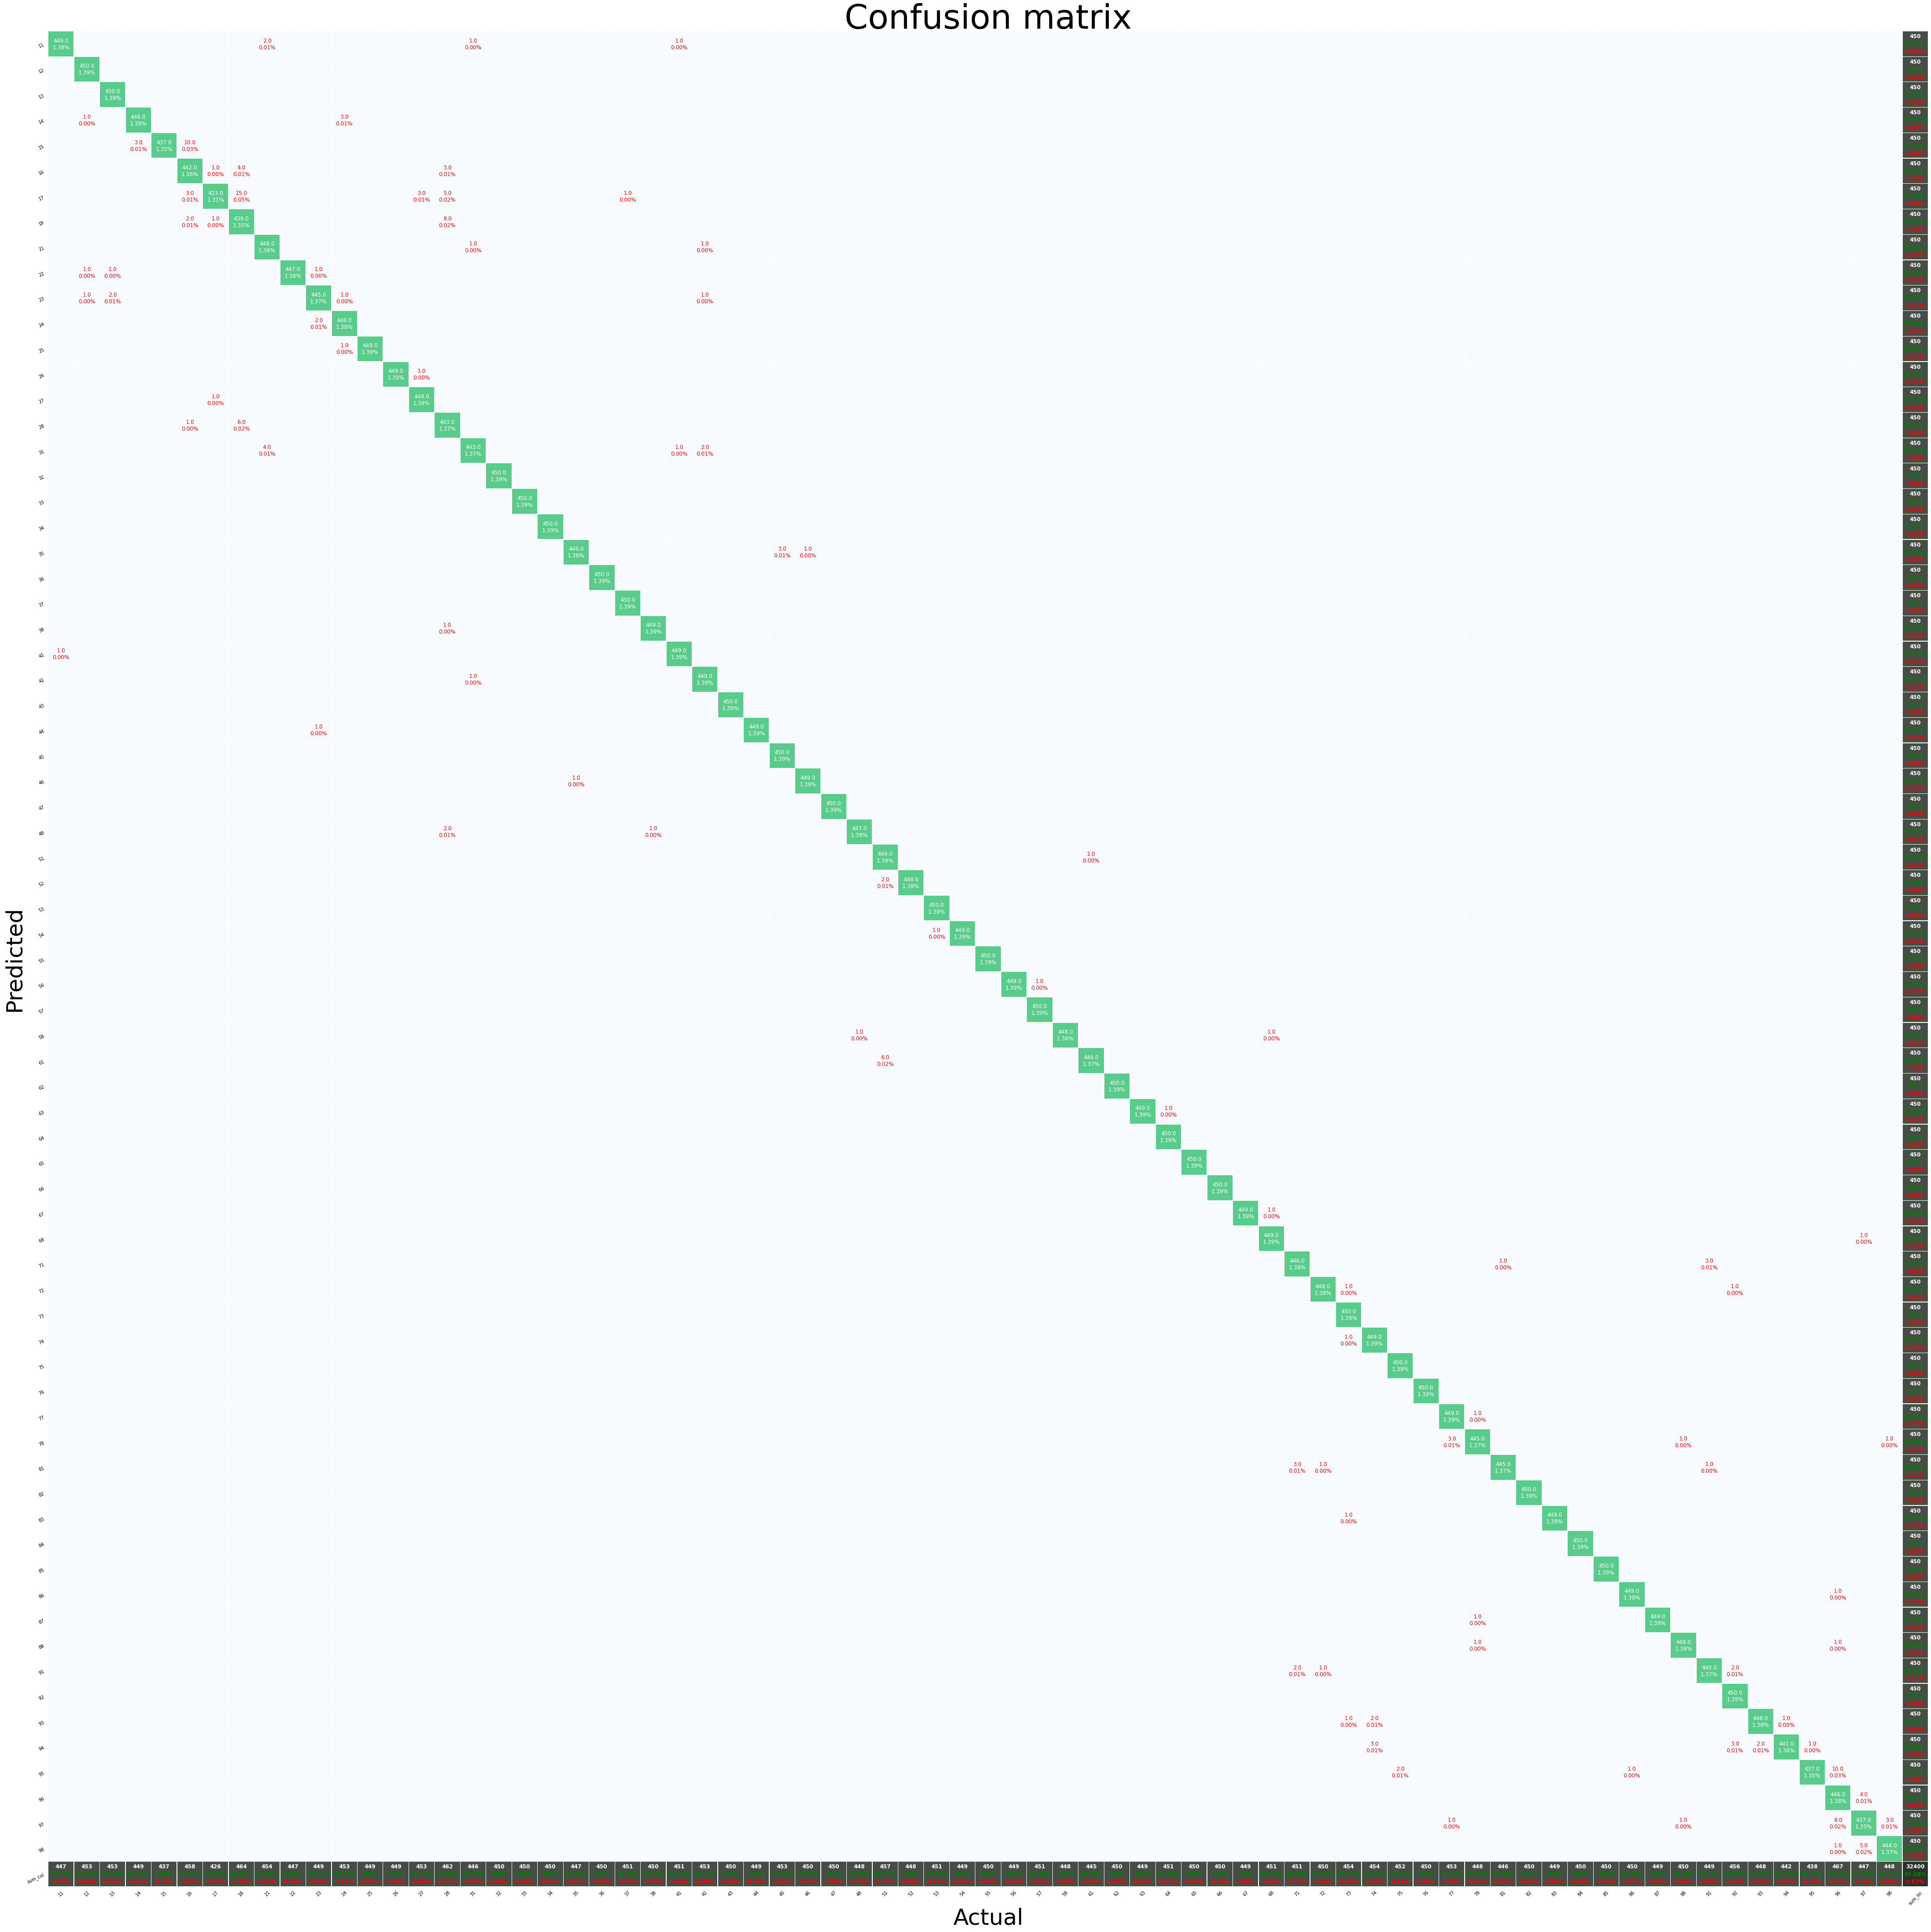
\includegraphics[width=150mm, angle=0]{4/Fotos/CM_A380_Sintetico.png}
    \captionsetup{justification=centering,margin=1.25cm}
    \caption{Matriz de confusión con los impactos sintéticos: \textbf{PRECISIÓN 99,38\%}}
    \label{fig:CM_Real}
\end{figure}

\begin{figure}[H]
    \centering
    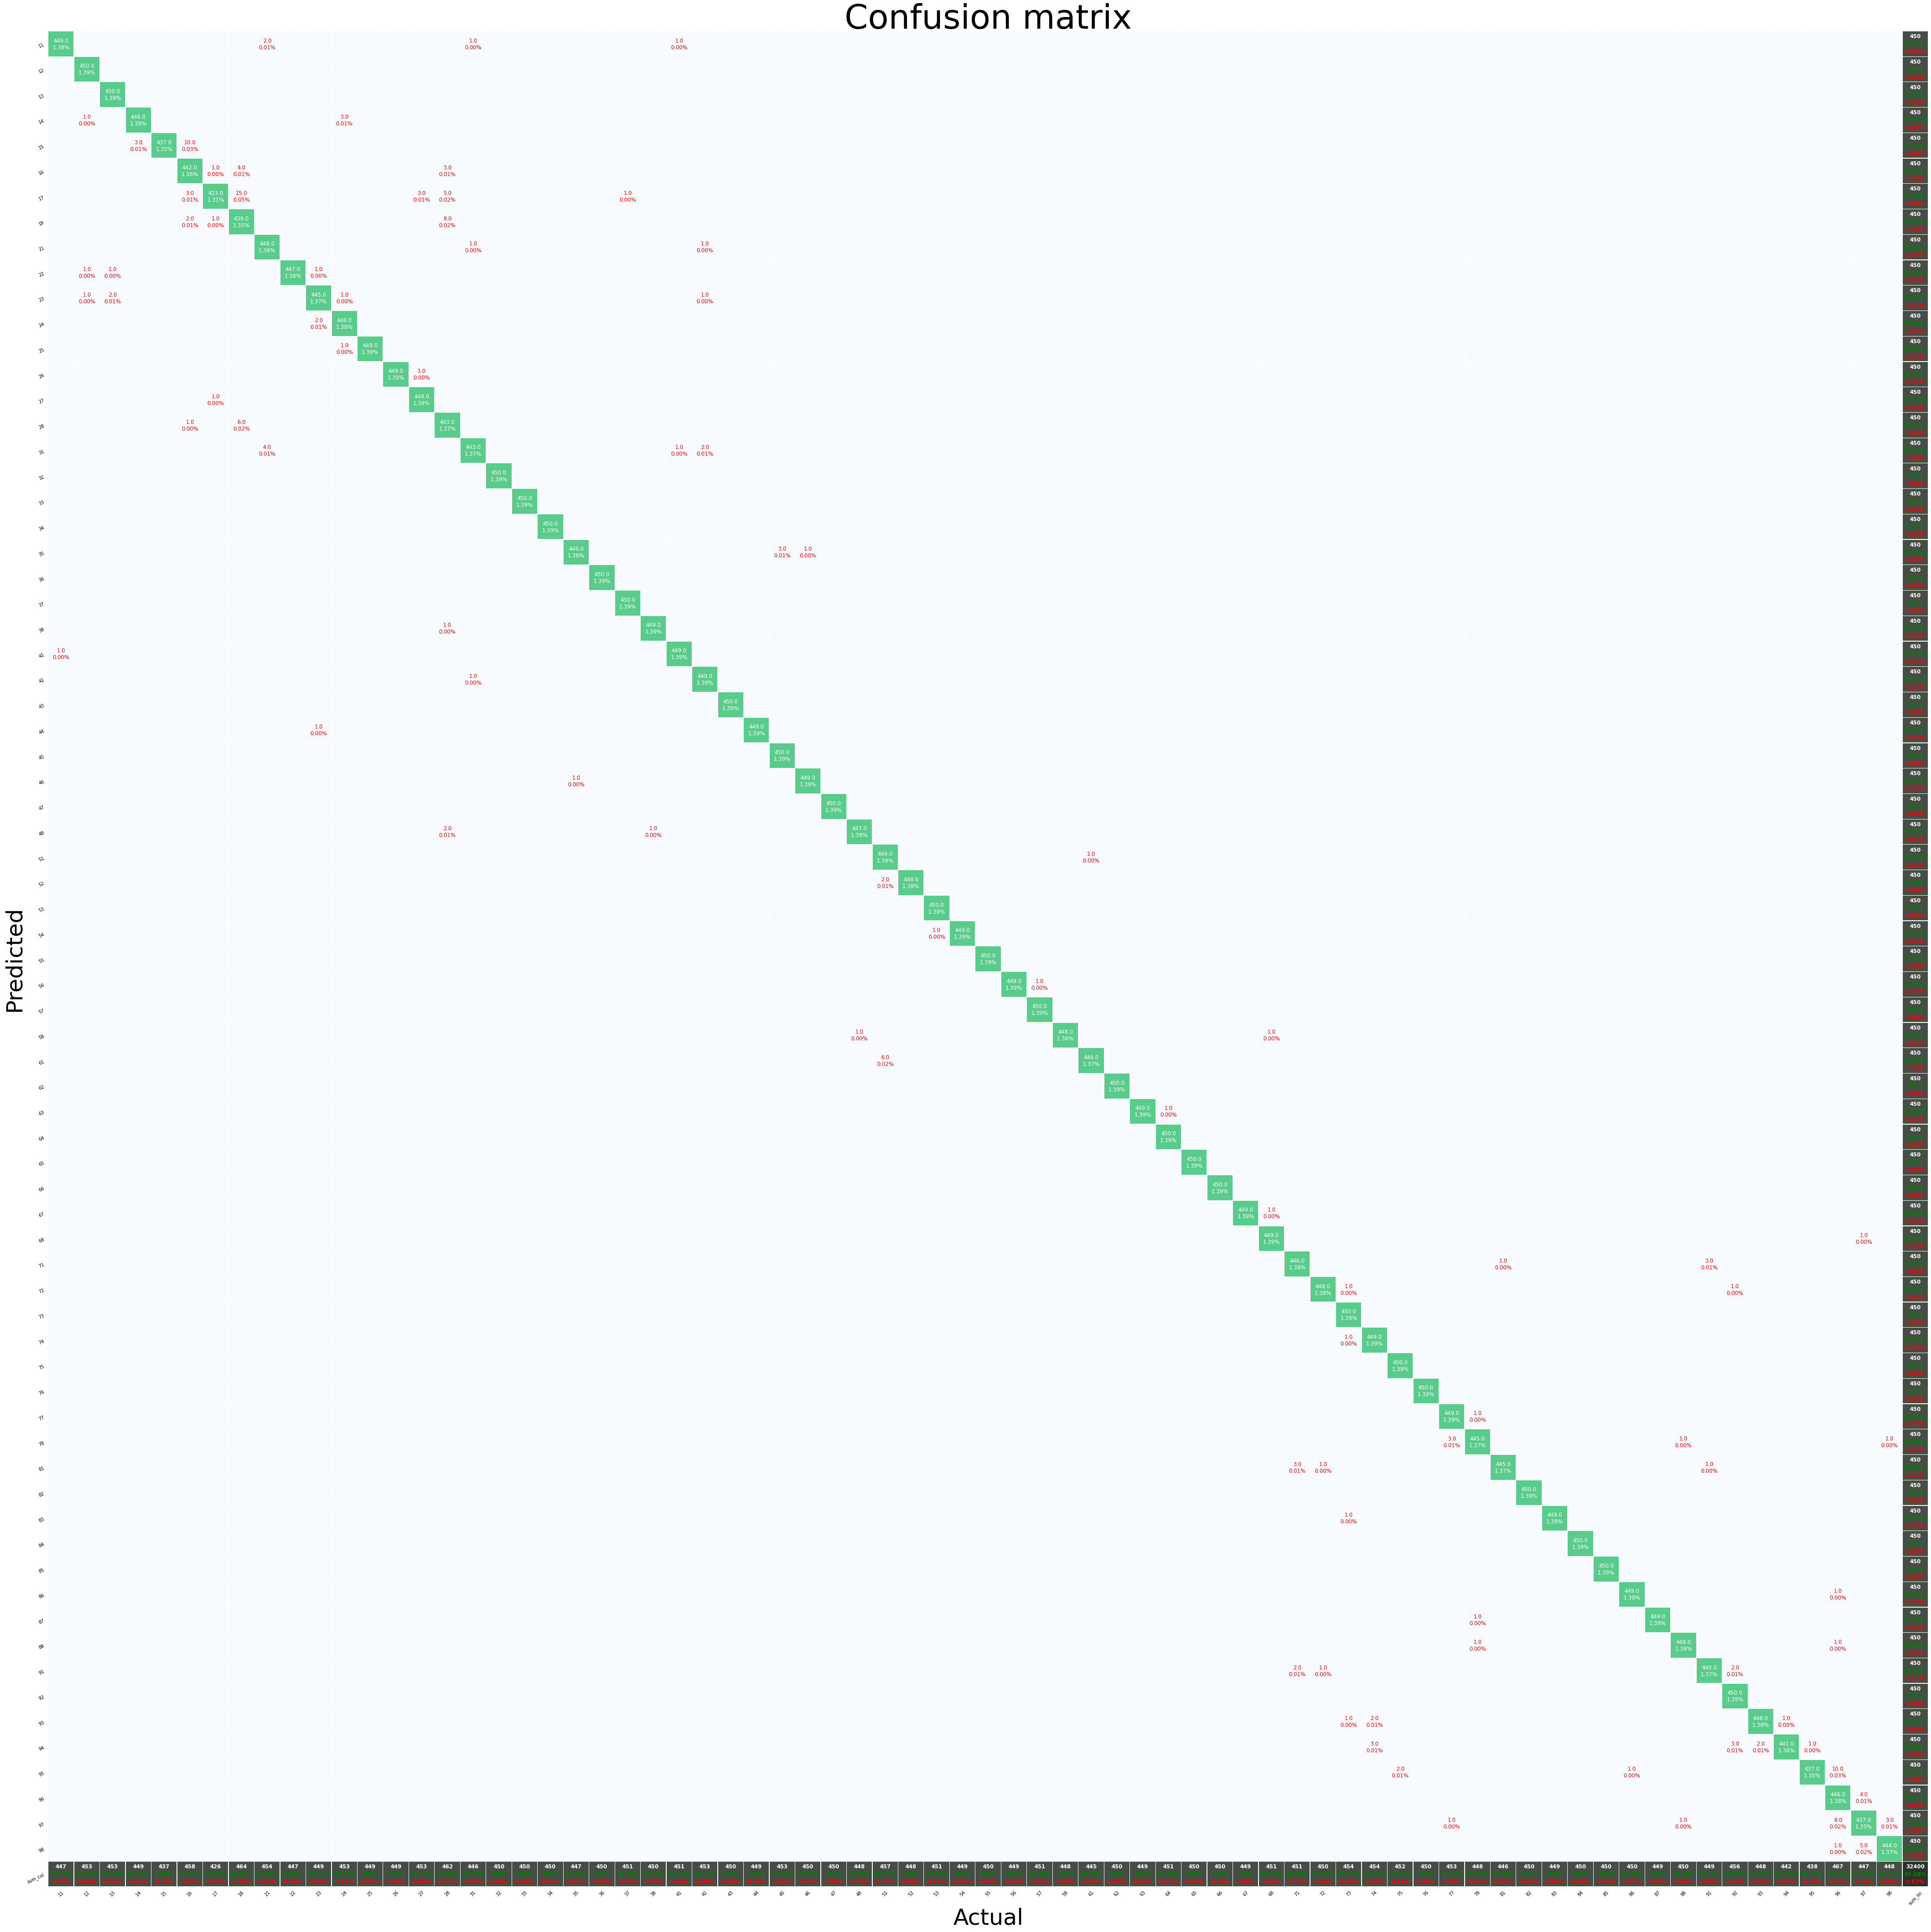
\includegraphics[width=150mm, angle=0]{4/Fotos/CM_A380_Sintetico.png}
    \captionsetup{justification=centering,margin=1.25cm}
    \caption{Matriz de confusión con los impactos reales: \textbf{PRECISIÓN 86,86\%}}
    \label{fig:CM_Sintetico}
\end{figure}

En la Figura \ref{fig:CM_Real} se puede comprobar que cuando entrenas una red con un determinado grupo de datos y lo validas con datos extraídos de la misma fuente, su precisión puede llegar a ser tan alta como la que se ha conseguido aquí.

Por otro lado, cuando se valida con un grupo de datos diferente al que se ha entrenado, su precisión cae. Sin embargo, en la Figura \ref{fig:CM_Sintetico} se muestra que la red entrenada con los datos sintéticos es capaz de clasificar con una precisión alta los datos reales.

\clearpage

%  --  --  %


\section{Caracterización de la energía}

CON DATOS DE CHRISTIAN Y AIRBUS AL MENOS

Red que clasifica la energía de impacto.

\clearpage

%  --  --  %


\section{Caracterización de la velocidad}

Si se termina por realizar el impactador, también se buscará una clasificacion de velocidad da impacto para diferentes masas y misma altura de suelta.

\clearpage

%  --  --  %


\section{Caracterización completa de un impacto}

Combinación de los anteriores clasificadores para comprobar la precisión completa de un impacto.

\clearpage